
\documentclass{beamer}
\usetheme{Darmstadt}
\usefonttheme[onlylarge]{structurebold}
\usepackage[T1]{fontenc}
\usepackage{t1enc}	
\usepackage{indentfirst}
\usepackage[utf8]{inputenc}
\usepackage[normalem]{ulem}
\usepackage[makeroom]{cancel}

\usepackage{graphicx}
\usepackage{graphics}
\usepackage{amssymb,amsmath}
\usepackage{animate}
\usepackage[super]{nth}
\usepackage[tight,footnotesize]{subfigure}
\usepackage{rotating}
\usepackage{bigstrut}

%EZT A CSOMAGOT MÉG ADD HOZZÁ!
\usepackage{multirow}

%\usepackage{subfig}
%\usepackage{wrapfig}
\linespread{1.5}


\newtheorem{tetel}{Tétel}
\DeclareMathOperator{\re}{Re}
\DeclareMathOperator{\im}{Im}
\DeclareMathOperator{\Span}{span}
\DeclareMathOperator{\thh}{th}
\DeclareMathOperator{\Hz}{Hz}
\DeclareMathOperator{\PLI}{PLI}
\DeclareMathOperator{\sgn}{sgn}
\DeclareMathOperator{\cur}{cur}
\DeclareMathOperator{\infx}{inf}
\DeclareMathOperator{\err}{err}
\DeclareMathOperator{\ido}{time}
\DeclareMathOperator{\grad}{grad}
\DeclareMathOperator{\intenzitas}{intenzitás}
\newcommand{\tss}[1]{\textsuperscript{#1}}
\newcommand{\IN}{\mathbb{N}}
\newcommand{\IZ}{\mathbb{Z}}
\newcommand{\IR}{\mathbb{R}}
\newcommand{\IC}{\mathbb{C}}
\newcommand{\ID}{\mathbb{D}}
\newcommand{\IT}{\mathbb{T}}
\newcommand{\IL}{\mathbb{L}}
\newcommand{\IH}{\mathbb{H}}
\newcommand{\IP}{\mathbb{P}}
\newcommand{\dt}{\ \mathrm{d}t}
\newcommand{\set}[2]{\left\{\, #1 \,:\, #2 \,\right\}}
\newcommand{\sset}[1]{\left\{\, #1 \,\right\}}
\newcommand{\conj}[1]{\overline{#1}}
\DeclareMathOperator{\arth}{arth}
\DeclareMathOperator{\tanhyp}{th}
\DeclareMathOperator{\dbest}{dbest}
\DeclareMathOperator{\PRD}{PRD}
\DeclareMathOperator{\CR}{CR}
\DeclareMathOperator{\QS}{QS}


\title{Biológiai jelek Hilbert-térbeli approximációja}
\author{Dózsa Tamás}
\institute{Programtervező Informatikus BSc \\ Eötvös Loránd  Tudományegyetem, Informatikai Kar\vspace{3mm}}
\date{\vspace{2mm}\\
\vspace{3mm}
\scriptsize
Budapest,\\ 2017. június x.
%\textcolor{blue}{The Project is supported by the European Union and co-financed by the European Social
%Fund (grant agreement no.\ T\'AMOP 4.2.2./B-10/1-2010-0030).}
}
\usetheme{Darmstadt} 
%\setbeamerfont{caption}{size=1pt}
\begin{document}

\begin{frame}
\titlepage
\end{frame}

\begin{frame}{Tartalomjegyzék}
\tableofcontents%[pausesection] % a szakaszok egymás után jelennek meg
\end{frame}


\section{Bevezetés}
\begin{frame}
\only<1>{
	\begin{block}{Motiváció}
	\begin{itemize}
		\item Az EKG elemzése nagy jelentőséggel bír az orvostudományban.
		\item Hosszú mérések, vagy több elvezetés esetén költséges a tárolás.
		\item A jel zajjal terhelt, ami nehezíti a pontos diagnózis felállítását.
		\item Hullámszegmensek meghatározása fontos probléma.
	\end{itemize}
\end{block}
	\begin{block}{Alkalmazások}
	\begin{itemize}
		\item \textbf{Tömörítés}
		\item Zajszűrés
		\item QRS detektálás
		\item Szívütések osztályozása
	\end{itemize}
\end{block}
}
\only<2>{
\begin{center}
   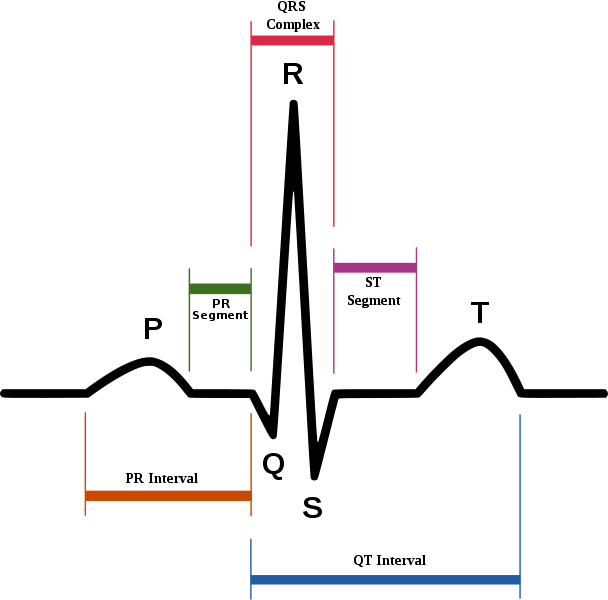
\includegraphics[scale=0.35]{./figures/ecg_wiki.png}
 		\label{fig:ekg}
\end{center}
}
\end{frame}

\begin{frame}{Approximáció Hilbert-terekben}
\only<1>{
\begin{block}{Definíciók}
	\begin{itemize}
		\item Legyen $(\mathcal{H},\left\langle .,.\right\rangle)$ Hilbert-tér, ahol
			\begin{equation*}
				\left\langle f,g\right\rangle := \int_{-\infty}^{\infty} f(t) g(t) \dt
			\end{equation*}
		\item $\set{\Phi_k}{0\leq k \leq n}$ ortonormált rendszer (ONR)
		\item Ortogonális projekció:
			\begin{equation*}
				S_n f:=\sum_{k=0}^{n} \left\langle f,\Phi_k\right\rangle \Phi_k
			\end{equation*}
	\end{itemize}
\end{block}
}
\only<2>{
	\begin{block}{Definíciók}
	\begin{itemize}
		\item Az approximáció hibája:
			\begin{equation*}
			\|f-S_nf\|^2=\|f\|^2-\sum_{k=0}^n|\langle f,\Phi_k\rangle|^2 \,.
			\end{equation*}
	\end{itemize}
	\end{block}
	\begin{block}{Feladat}
		\begin{itemize}
		  \item EKG esetén másodpercenként több száz adat keletkezik.
			\item A dolgozat célja a jel \textbf{tömörítése.}
			\item Ezért véges dimenziós altereket használunk (Euklideszi tér).
		\end{itemize}
	\end{block}
}
\end{frame}

\section{Előzmények}

\begin{frame}{Hermite-polinomok}
\linespread{1.0}
\begin{block}{Definíció}
	\begin{itemize}
		\item Rekurzió:
			\begin{equation*}
				\begin{split}
					&H_n(x)=2xH_{n-1}(x)-2(n-1)H_{n-2}(x)\quad (n\ge 2)\\
					&H_{-1}(x)=0,\  H_0(x)=1,\ \ H_1(x)=2x
				\end{split}
			\end{equation*}
		\item Ortogonalitás:
			\begin{gather*}
				\begin{split}
					\langle H_n,H_m\rangle_{\rho}:&=\int_{-\infty}^\infty H_n(t) H_m(t)\rho(t) \dt\\
					\langle H_n,H_m\rangle_{\rho} &= 0 \quad (n \neq m)
				\end{split}
			\end{gather*}
		\item Súlyfüggvény:
			\begin{equation*}
				\rho(t) := e^{-t^2}
			\end{equation*}
	\end{itemize}
\end{block}
\end{frame}


\begin{frame}{Hermite-függvények}
\only<1>{
\begin{block}{Definíció}
		\begin{equation*}
			\Phi_n(x):=H_n(x)e^{-x^2/2}/\sqrt{\pi^{1/2}2^n n!} \quad (n\in\Bbb N, x\in\Bbb R)
		\end{equation*}
\end{block}
\begin{figure}
  \centering
\subfigure[$\Phi_{0}(x)$]{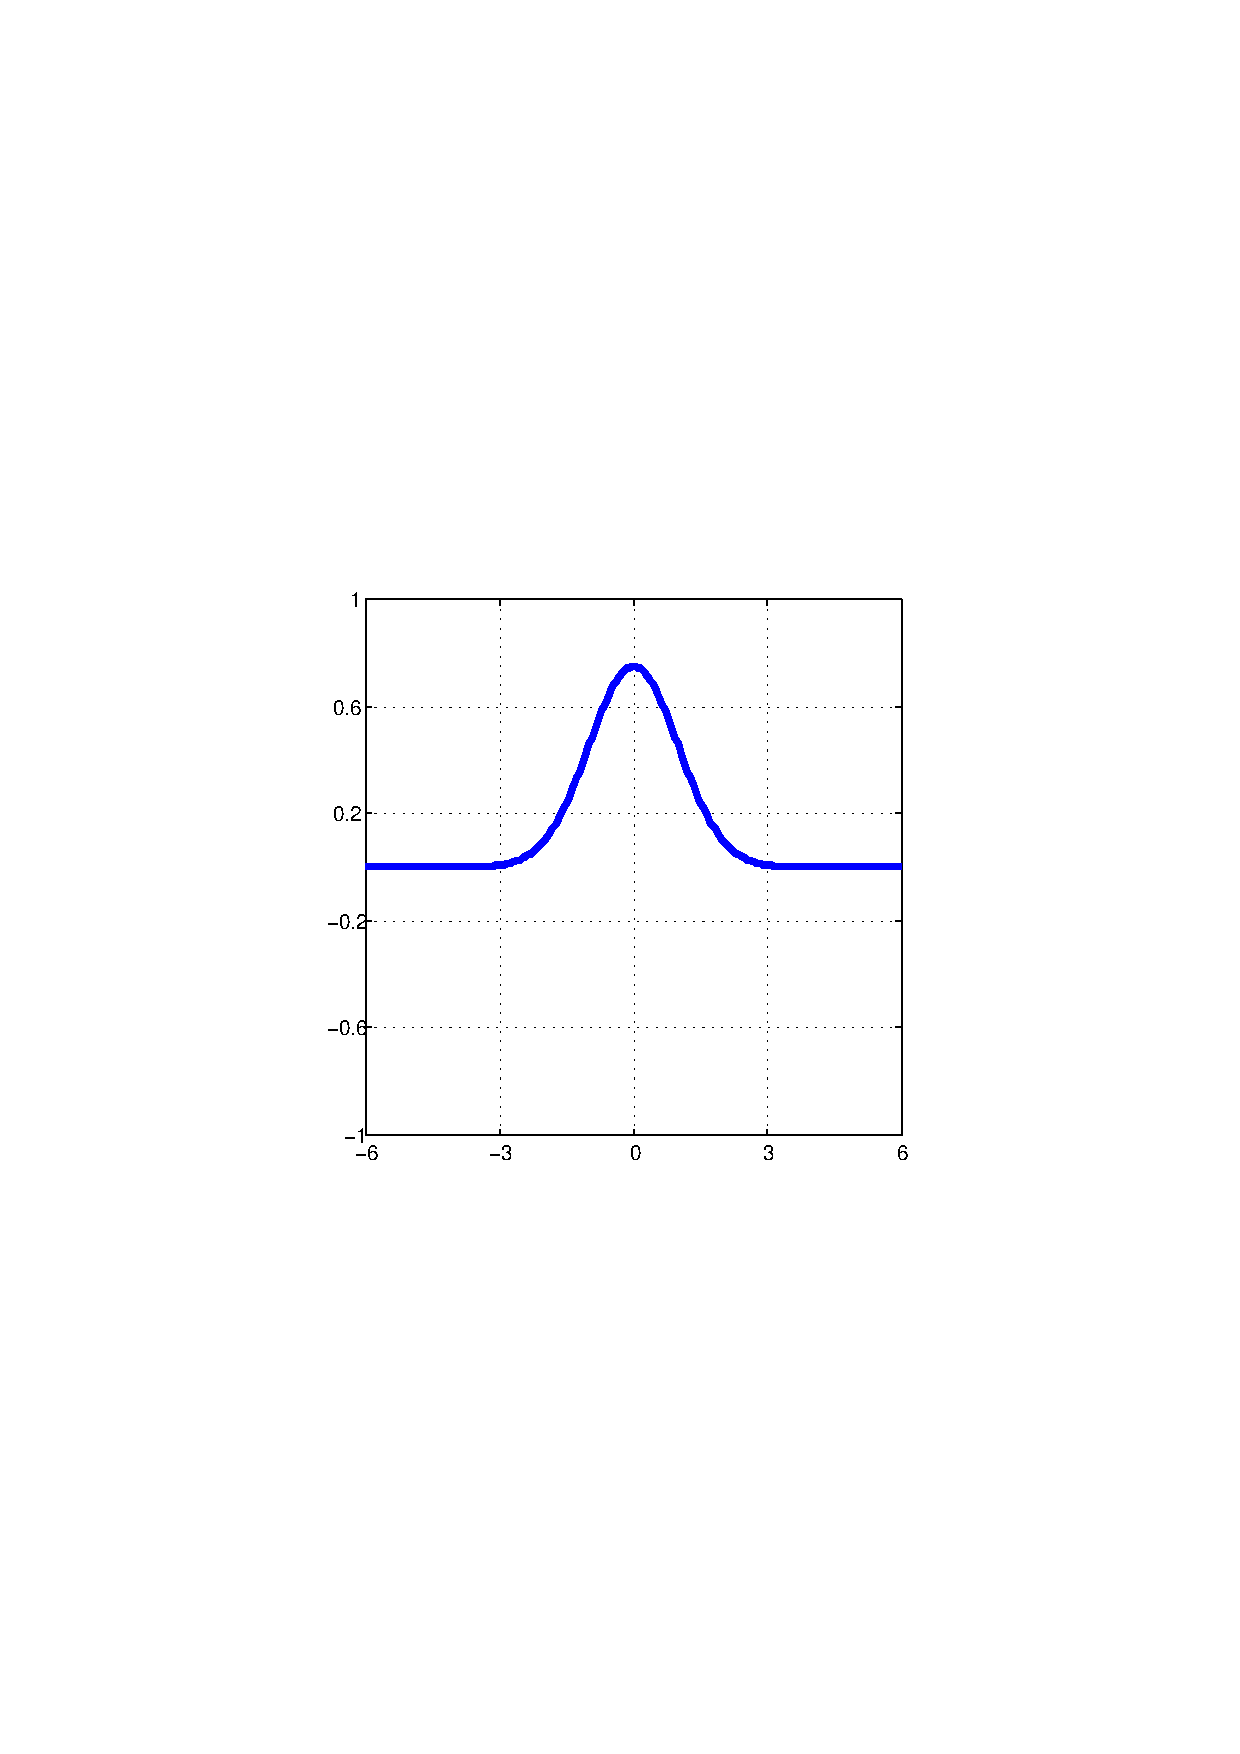
\includegraphics[scale=0.3,trim=150 280 150 280,clip]{./figures/phi0.pdf}} 
\subfigure[$\Phi_{1}(x)$]{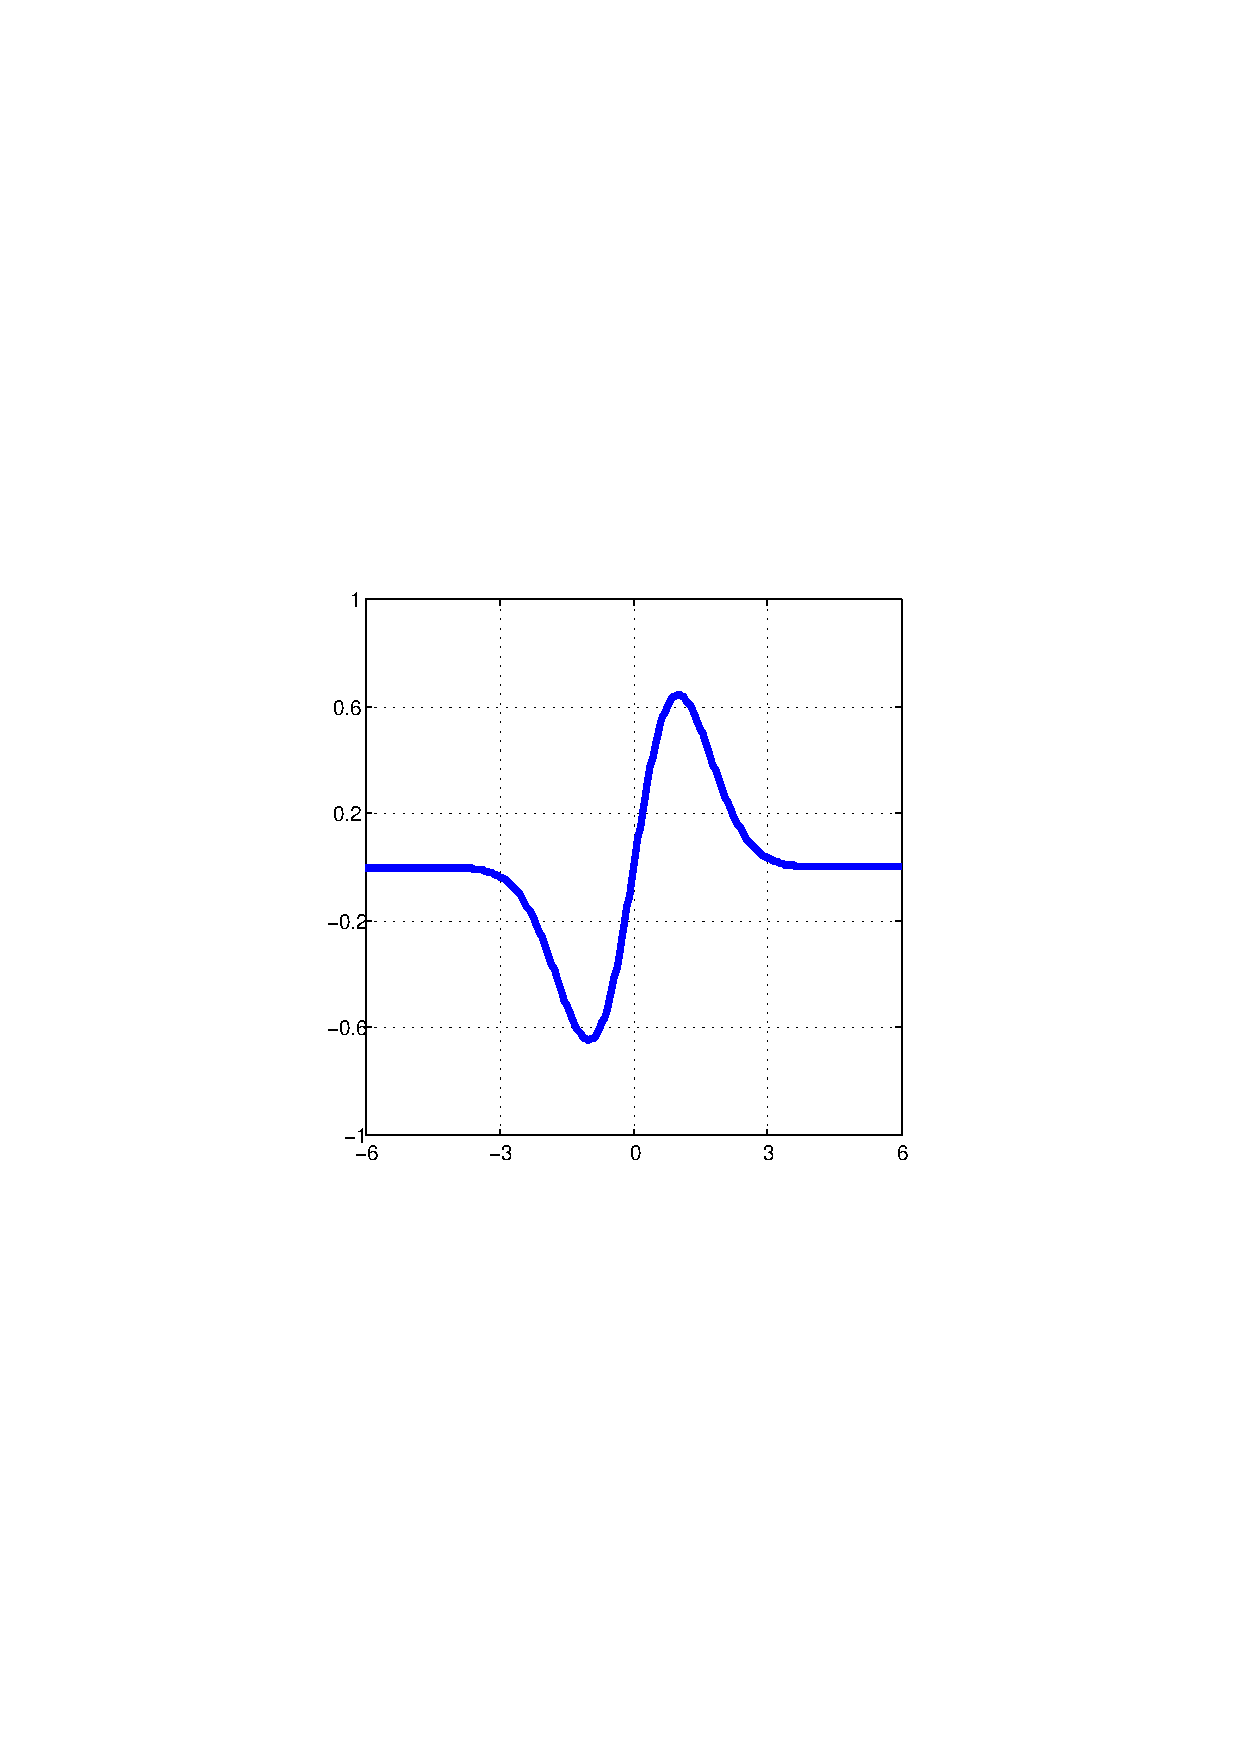
\includegraphics[scale=0.3,trim=150 280 150 280,clip]{./figures/phi1.pdf}}
\subfigure[$\Phi_{2}(x)$]{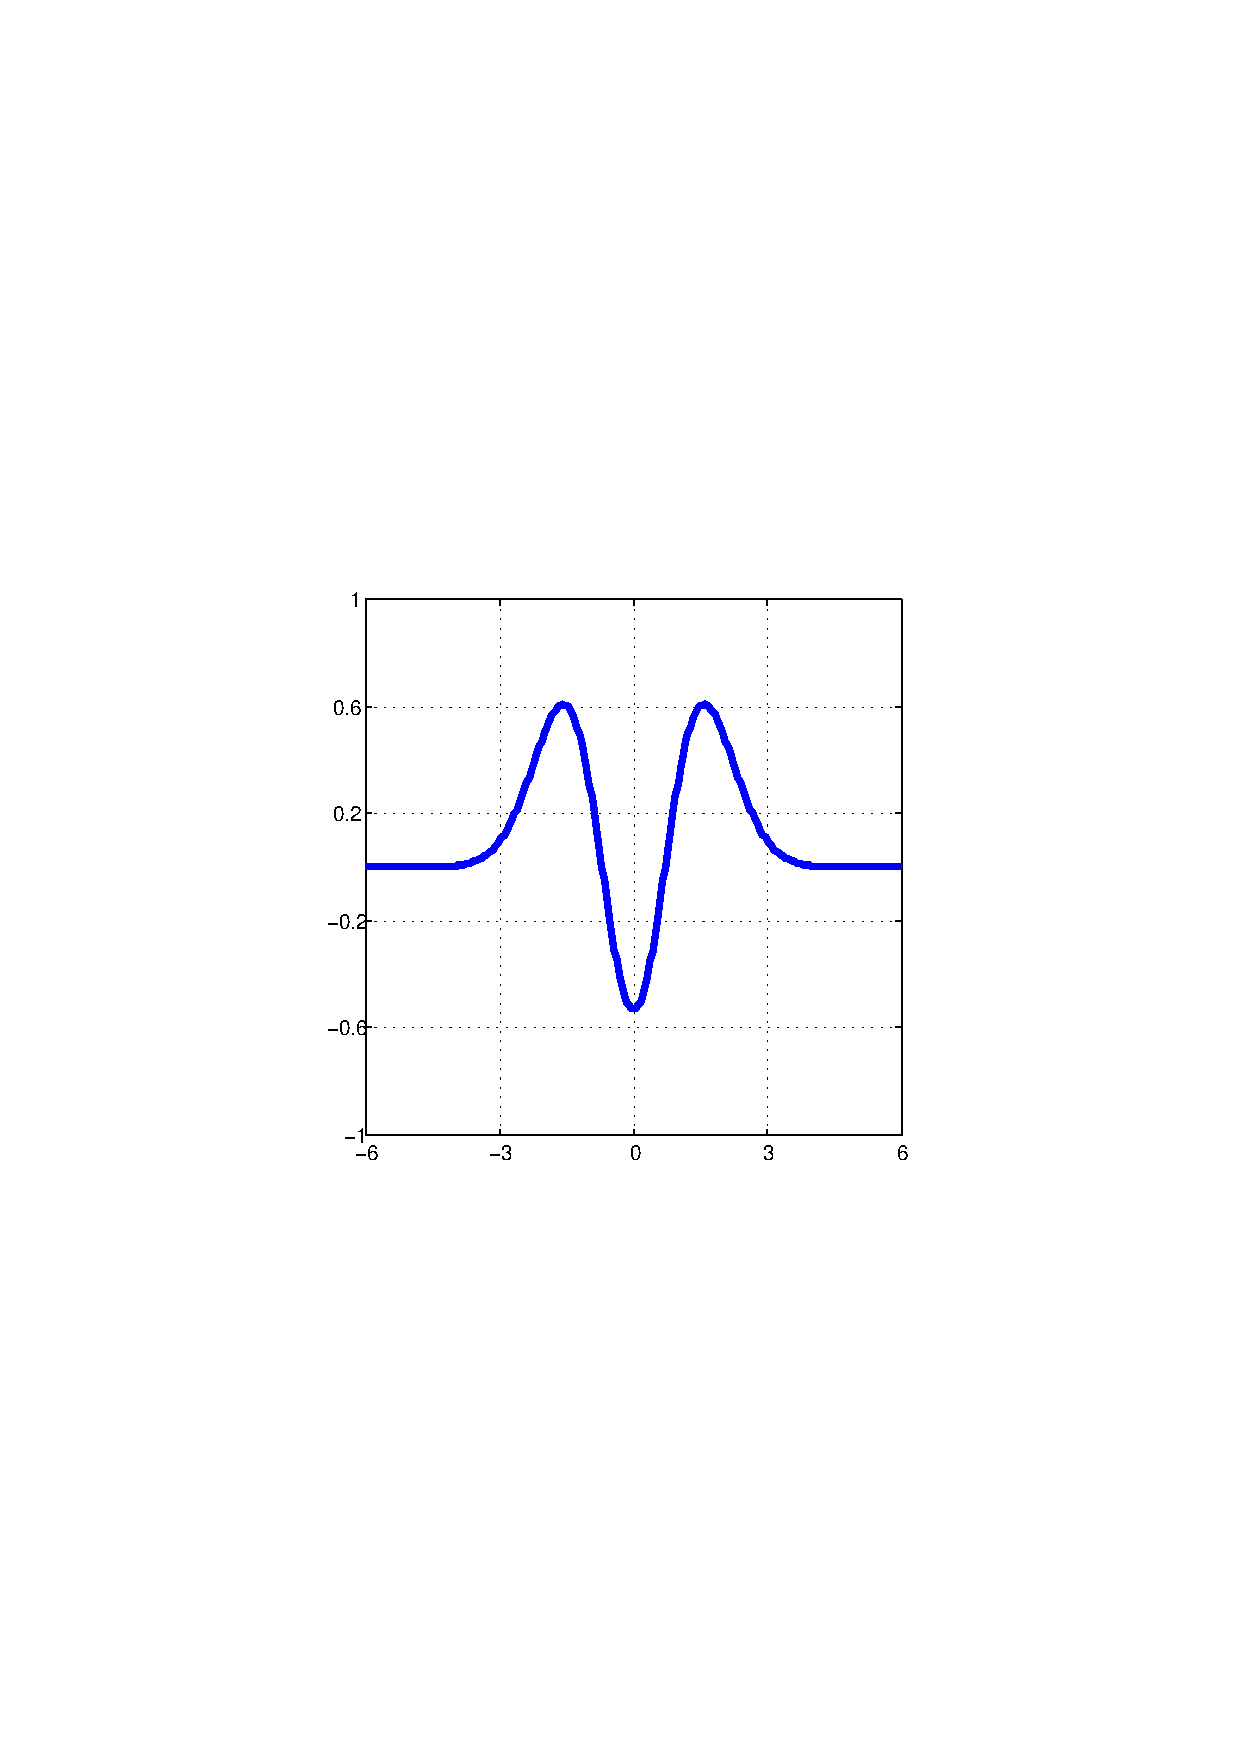
\includegraphics[scale=0.3,trim=150 280 150 280,clip]{./figures/phi2.pdf}} 
\caption{A Hermite-f\"uggv\'enyrendszer első három tagja.}
\label{fig:phi0-3}
\end{figure}

}
\only<2>{
	\begin{block}{Tulajdonságok}
	\begin{itemize}
		\item ONR
		\item Gyorsan tartanak 0-hoz:
			\begin{equation*}
				|\Phi_n(x)|\le M_n e^{-x^2/4}\le M_n \quad (x\in\Bbb R, n\in\Bbb N)
			\end{equation*}
		\item	Stabil, másodrendű rekurzió:
			\begin{equation*}
				\begin{split}
					&\Phi_n(x)=\sqrt{\frac 2 n}x\Phi_{n-1}-\sqrt{\frac {n-1} n}\Phi_{n-2}(x)\quad (n\ge 2)\\ 
					&\Phi_0(x)=e^{-x^2/2}/\pi^{1/4},\ \Phi_1(x)= \sqrt 2 x e^{-x^2/2}/\pi^{1/4}\quad (x\in\Bbb R)
				\end{split}
			\end{equation*}	
	\end{itemize}
	\end{block}
}
\only<3>{
\linespread{1.0}
	\begin{block}{Tulajdonságok}
	\begin{itemize}
		\item $\Phi_n$ deriváltja:
			\begin{equation*}
				\Phi'_n(x)=\sqrt{2n}\Phi_{n-1}(x)-x\Phi_n(x) \quad (n\ge 0, x\in\Bbb R)
			\end{equation*}
		\item	Alakjuk korrelál az EKG-vel.
		\item Korábbi cikkek is használták \footnotemark[1] \footnotemark[2].
	\end{itemize}
	\end{block}
\footnotetext[1]{R. Jane, S. Olmos, P. Laguna, and P. Caminal, \textit{Adaptive Hermite models for ECG data compression: Performance and evaluation with automatic wave detection}, in Proc. of the Int. Conf. on Comp. in Card., 1993, pp. 389--392. \vspace{3mm}}	
\footnotetext[2]{A. Sandryhaila, S. Saba, M. Püschel, and J. Kovacevic, \textit{Efficient compression
of QRS complexes using Hermite expansion}, IEEE Trans. on Sig. Proc., vol. 60, no. 2, pp. 947–955, 2012. \vspace{3mm}}	
}
\end{frame}

\section{Kidolgozott módszer}

\begin{frame}{Rendszerek affin transzformáltja}
\only<1>{
	\begin{block}{Ötlet}
	\begin{itemize}
		\item Transzlációs, és dilatációs paraméterek bevezetése:
			\begin{equation*}
				\Phi_k^{a,\lambda}(x):=\Phi_k(\lambda x+a) \quad  (x,a\in\Bbb R, \lambda>0)\,.
			\end{equation*}
		\item	$\set{\sqrt{\lambda}\Phi_k^{a,\lambda}}{0\leq k \leq n}$ is ONR.
		\item Legjobb közelítés:
			\begin{equation*}
				S_n^{a,\lambda}f:=\sum_{k=0}^n\langle f,\Phi_k^{a,\lambda}\rangle\Phi_k^{a,\lambda}\quad
			(n\in\Bbb N, a\in\Bbb R,\lambda>0)\,.
			\end{equation*}
			\item Implementációs szempontok miatt $f^{a,\lambda}$-t használjuk.
	\end{itemize}
	\end{block}
}
\only<2>{
\linespread{1.0}
	\vspace{-2mm}
	\begin{block}{Célfüggvény definíciója}
	\begin{itemize}
		\item A Bessel egyenlőtlenség alapján a hibaformula:
			\begin{equation*}
				D^2_n(a,\lambda):=\|f\|^2-\sum_{k=0}^n|\langle f,\Phi_k^{a,\lambda}\rangle|^2\,.
			\end{equation*}
		\item Használható továbbá a
			\begin{equation*}
				F_n(a,\lambda):=\sum_{k=0}^n|\langle f,\Phi_k^{a,\lambda}\rangle|^2\,.
			\end{equation*}
	\end{itemize}
	\end{block}
	\begin{block}{Problémák}
	\begin{itemize}
		 \item Létezik-e a hibafüggvényeknek minimum, maximum helye?
		 \item Nem triviális: az értelmezési tartomány nem kompakt halmaz.
	\end{itemize}
	\end{block}	
}
\end{frame}

\begin{frame}{Optimalizációs módszerek}
\only<1>{
	\begin{block}{Cél}
		A legjobb transzlációs, dilatációs paraméterek megtalálása.
	\end{block}
	\begin{block}{Módszerek}
		\begin{itemize}
			\item Determinisztikus:
				 \begin{itemize}
						\item Gradiens módszer (parciális deriváltak szükségesek)
						\item \textbf{Nelder--Mead (NM) szimplex alapú módszer} 
				 \end{itemize}
			\item Nem determinisztikus:
				 \begin{itemize}
						\item Particle Swarm Optimization (PSO), raj alapú optimalizáció
				 \end{itemize}
		\end{itemize}
	\end{block}	
}
\end{frame}


\begin{frame}{Matching Pursuit algoritmus}
\only<1>{
	\begin{block}{Cél}
		\begin{itemize}
			\item Egy szívütés – több függvényrendszer.
			\item Mohó algoritmus, minden körben a hibafüggvény minimumát keresi (a reziduum jelre nézve).
		\end{itemize}
	\end{block}	
	\begin{block}{Előnyök}
		\begin{itemize}
			\item Alkalmas a szegmensek detektálására.
			\item Adaptív reprezentáció.
			\item Pontosabb approximáció kevesebb együtthatóval.
			\item A dolgozatban használt együtthatók száma: 7, 6, 2 .
		\end{itemize}
	\end{block}		
}
\only<2>{
	\begin{figure}
  \animategraphics[autoplay,loop,scale=0.45,trim=100 210 100 260]{4}{./Animation/hermiteECG_}{0}{50}\vspace{-2mm}
		\caption{QRS paramétereinek optimalizációja.}
	\end{figure}	
}
\only<3>{
	\begin{figure}
  \animategraphics[autoplay,loop,scale=0.45,trim=100 210 100 260]{4}{./Animation/hermiteECG_}{107}{157}\vspace{-2mm}
		\caption{T paramétereinek optimalizációja.}
	\end{figure}	
}
\only<4>{
	\begin{figure}
  \animategraphics[autoplay,loop,scale=0.45,trim=100 210 100 260]{4}{./Animation/hermiteECG_}{246}{296}\vspace{-2mm}
		\caption{P paramétereinek optimalizációja.}
	\end{figure}	
}
\only<5>{
\begin{figure}[htb!]
  \centering
\subfigure[A QRS approxim\'aci\'oja.]{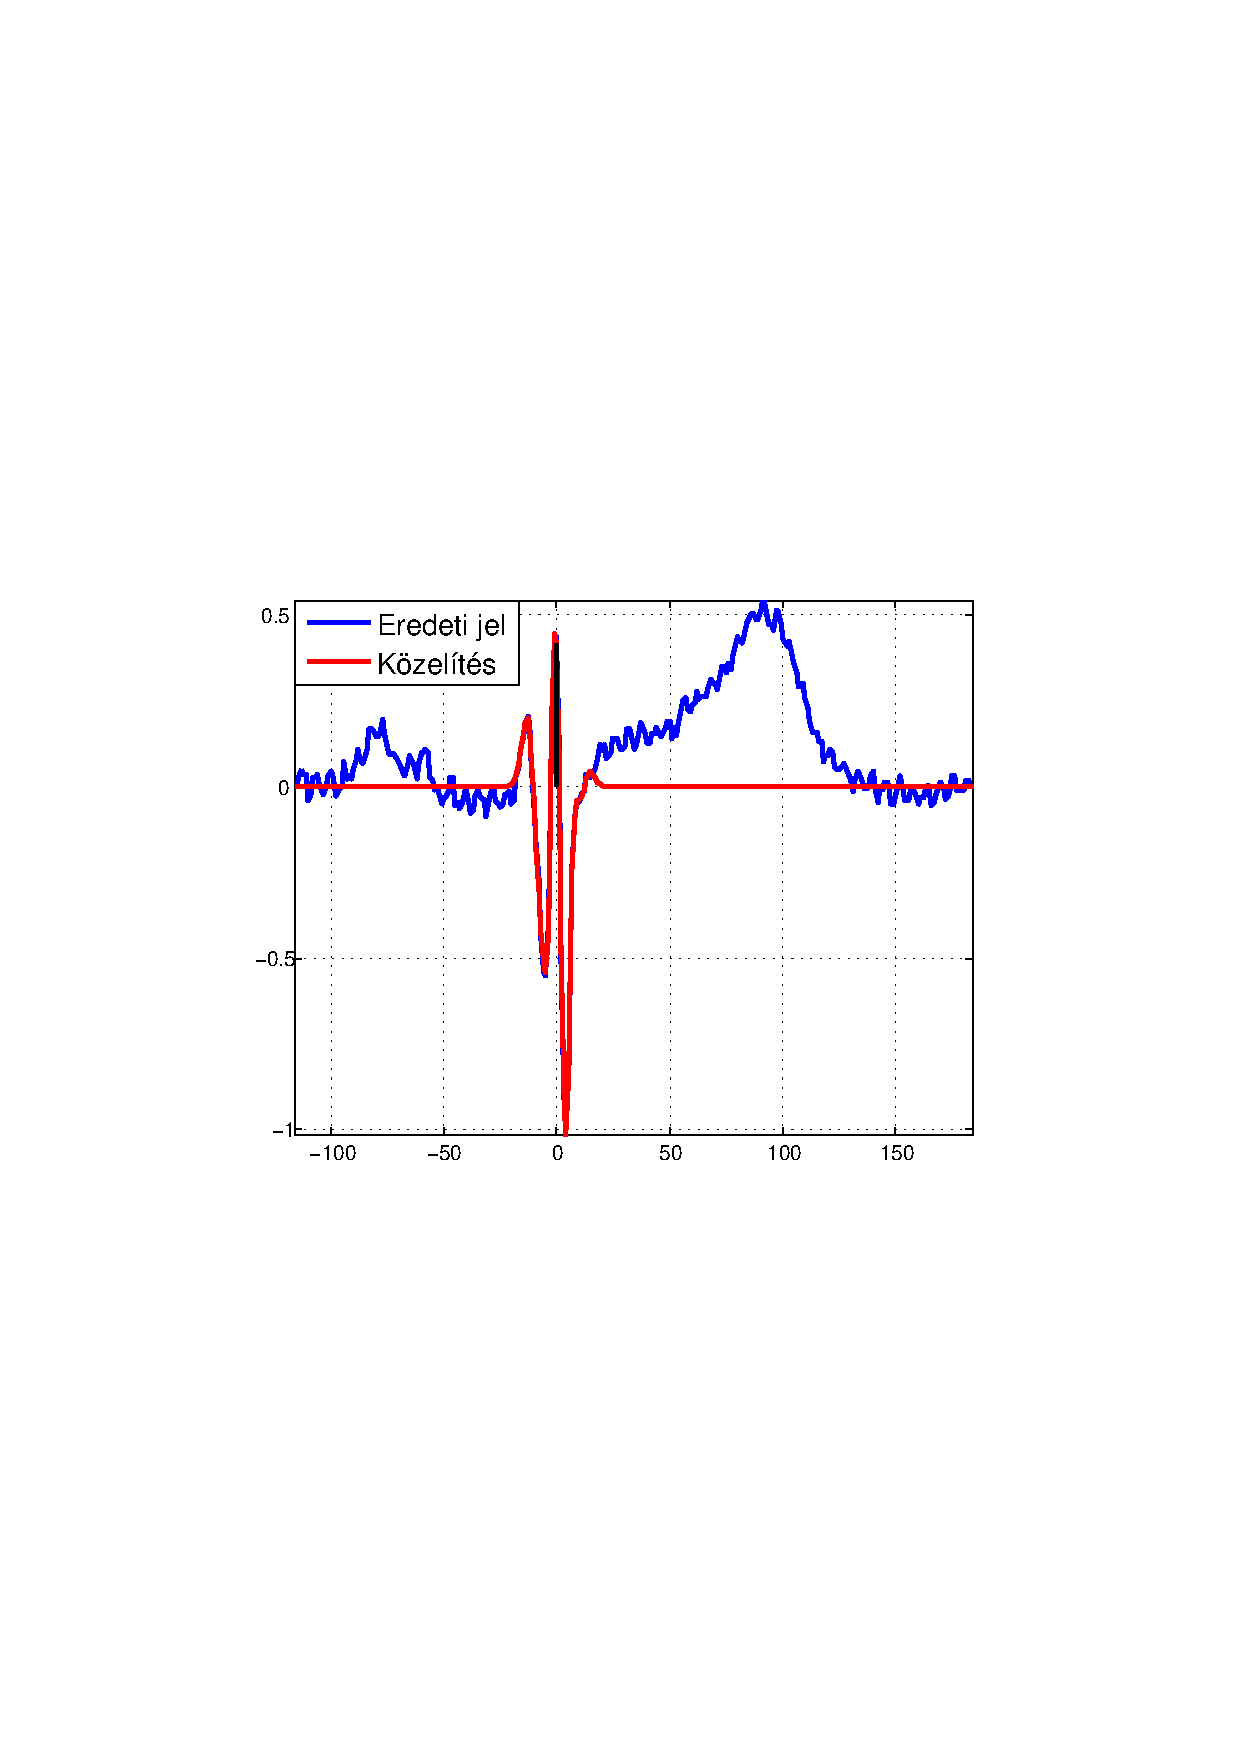
\includegraphics[scale=0.4,trim=120 280 100 280,clip]{./figures/abra_lepes0.pdf}} 
\subfigure[A T hull\'am approxim\'aci\'oja.]{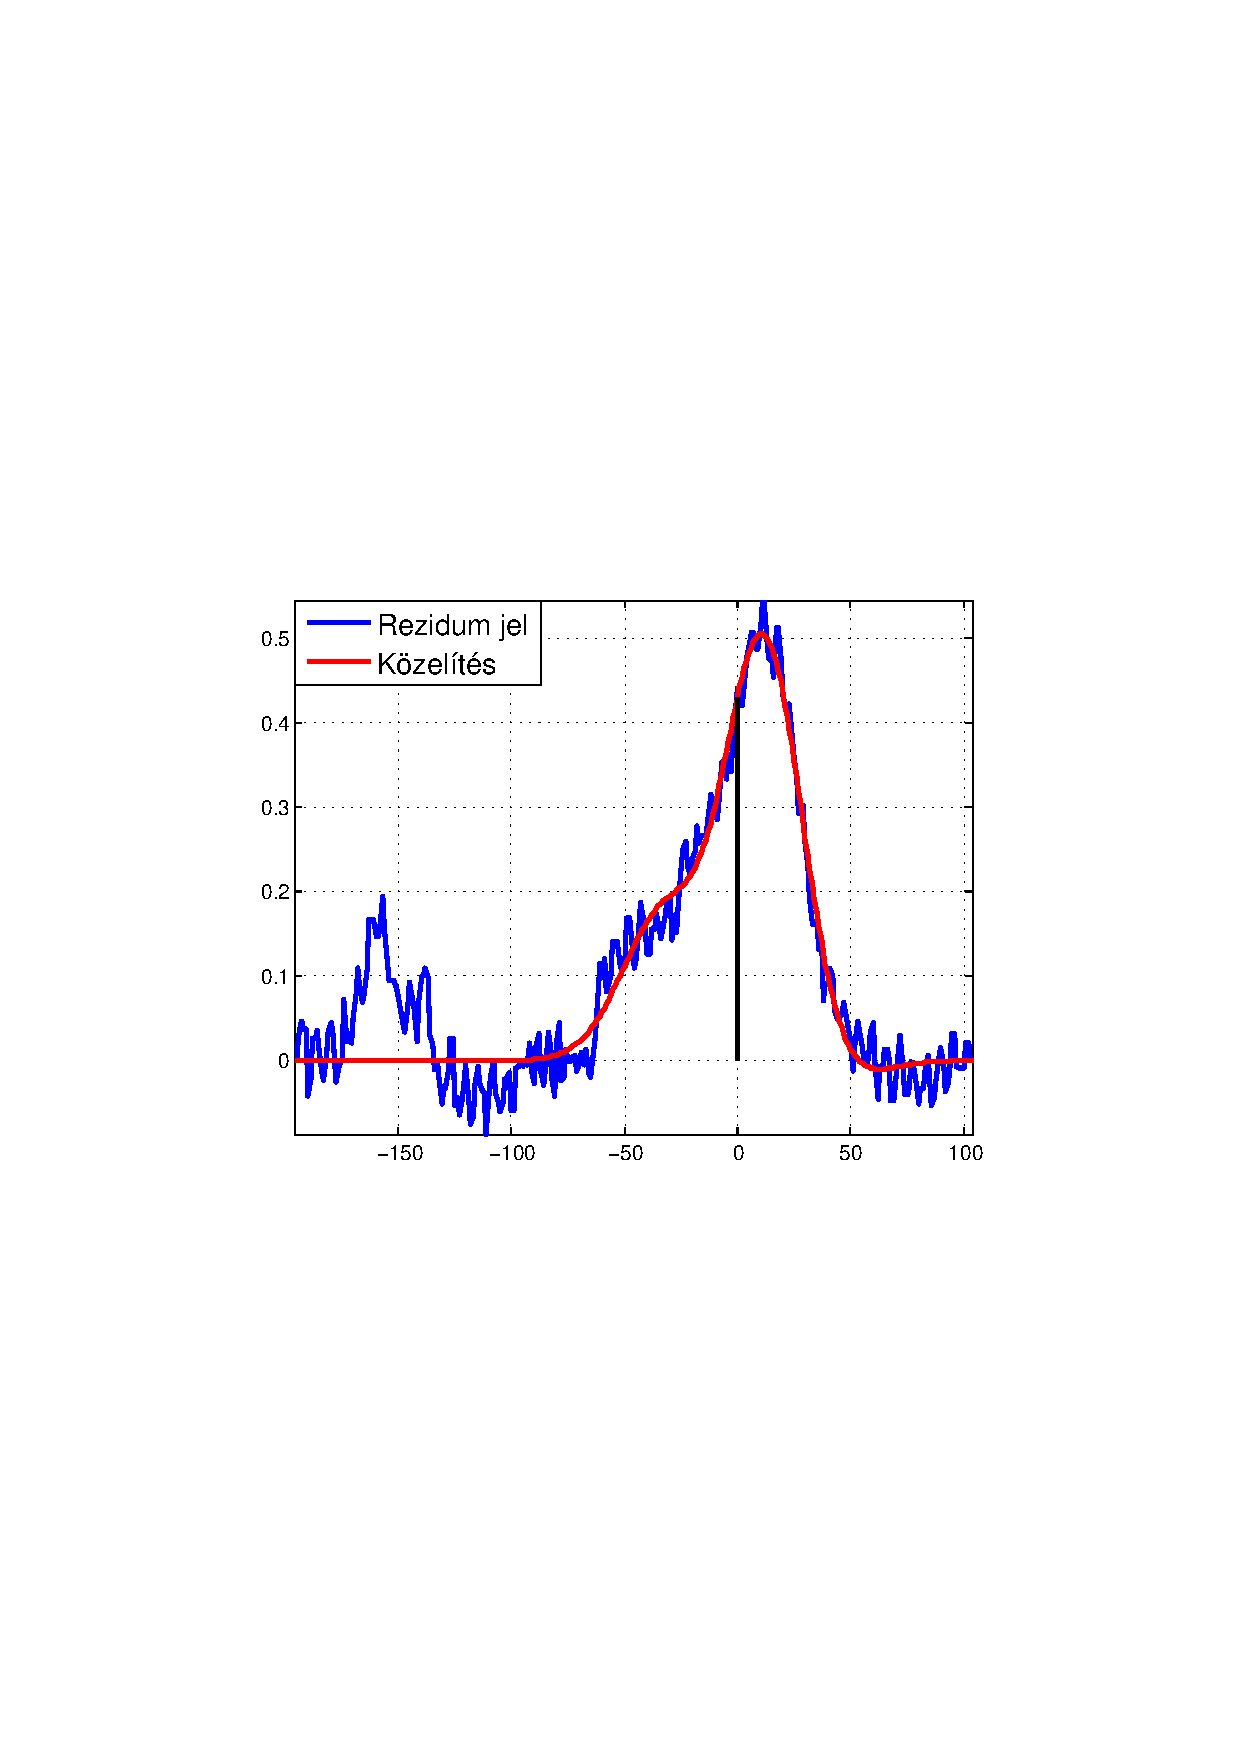
\includegraphics[scale=0.4,trim=120 280 100 280,clip]{./figures/abra_lepes1.pdf}}
\caption{Az MP algoritmus lépései (1-2).}
\end{figure}
}
\only<6>{
\begin{figure}[htb!]
  \centering
\subfigure[A P hull\'am approxim\'aci\'oja.]{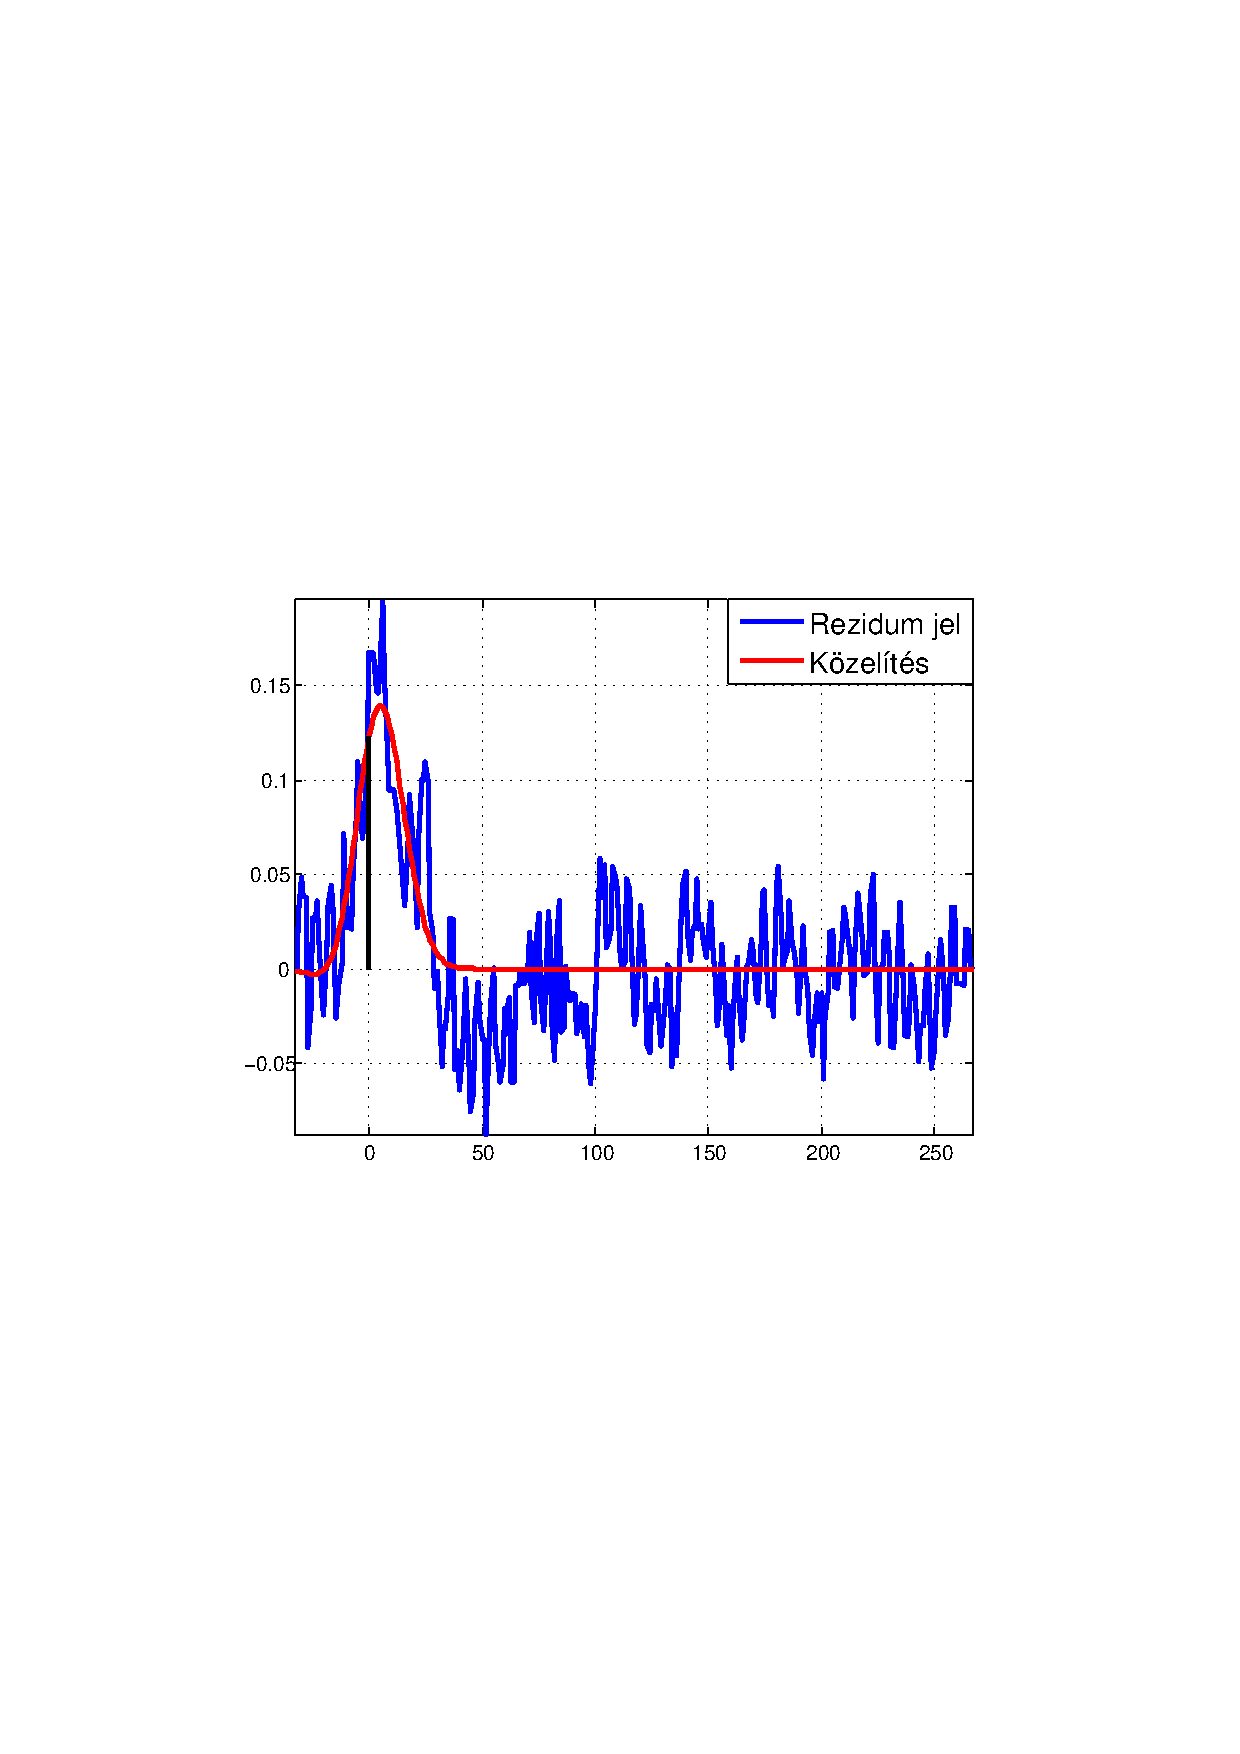
\includegraphics[scale=0.4,trim=120 280 100 280,clip]{./figures/abra_lepes2.pdf}} 
\subfigure[Szeparált szívütés.]{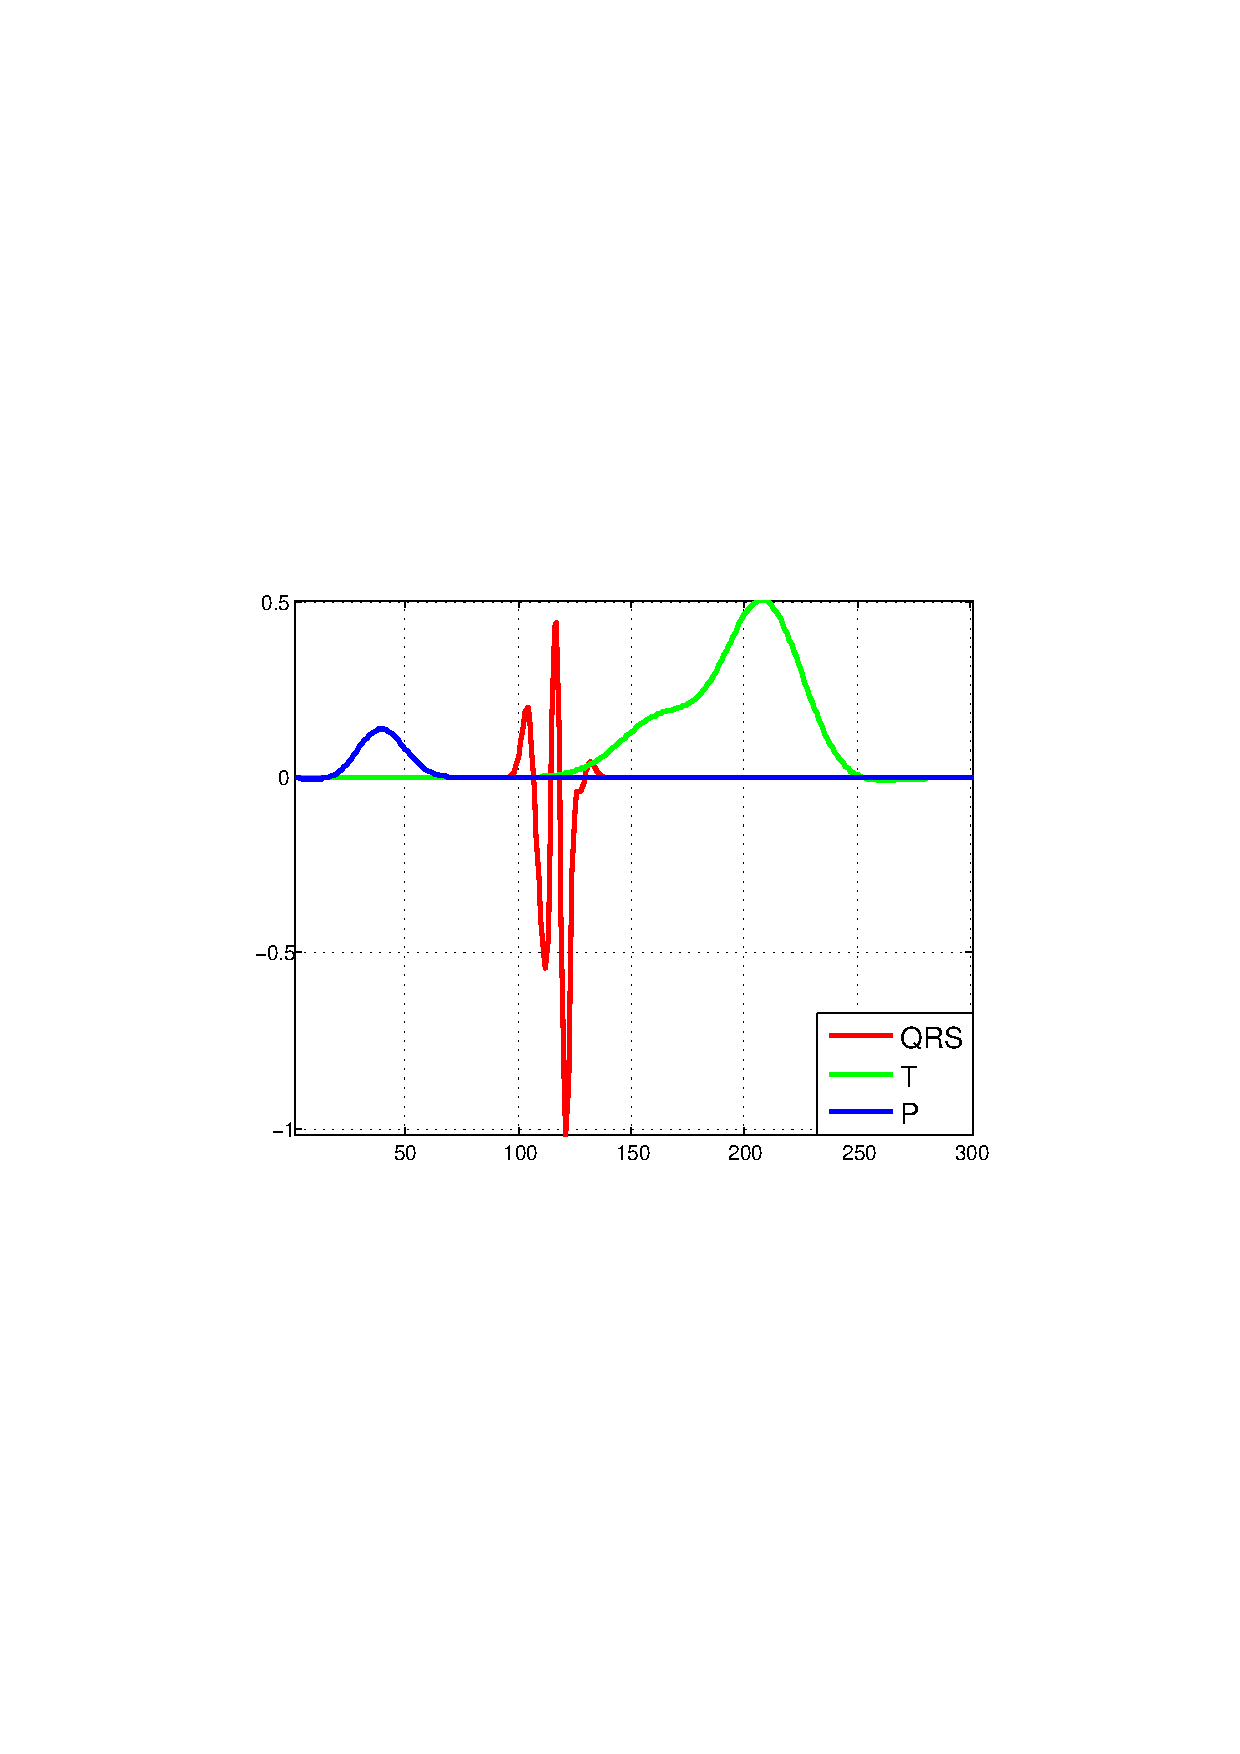
\includegraphics[scale=0.4,trim=120 280 100 280,clip]{./figures/abra_lepes3.pdf}}
\caption{Az MP algoritmus lépései (3-4).}
\end{figure}
}
\end{frame}

\section{Implementáció}
\label{tab:implemenation}
\begin{frame}{Megvalósítás}
\linespread{0.8}
\small
\vspace{-2mm}
\begin{block}{Felépítés}
	\begin{itemize}
		\item c++ nyelven megírt jelfeldolgozó rész.
		\item Webes felhasználói felület.
	\end{itemize}
	\end{block}
			
\end{frame}

\begin{frame}{A tömörítés implementációja}
\linespread{0.8}
\small
\vspace{-2mm}
\begin{block}{Modulok}
	\begin{itemize}
		\item Objektum orientált felépítés.
		\item Jól definiált interfészek.
		\item Elkülönített szolgáltatások.
		\item Újrafelhasználhatóság, könnyen bővíthetőség.
	\end{itemize}
	\end{block}		
	
\end{frame}

\begin{frame}{A tömörítés implementációja}
\linespread{0.8}
\small
\vspace{-2mm}
\begin{block}{Alkalmazott technikák, érdekességek}
	\begin{itemize}
		\item Összesen 9 c++ nyelven megírt modul.
		\item Algoritmusok: Nelder-Mead, MP, Hermite függvény gyökeinek megtalálása.
		\item c++ 11 adottságainak felhasználása: lambda függvények. 
	\end{itemize}
	\end{block}		
	
\begin{block}{A hatékonyság szem előtt tartása}
	\begin{itemize}
		\item Dinamikus memória használata (Hermite rendszerek).
		\item c++ sajátottságainak kihasználása, adatábrázolás során.
		\item A Standard Library szolgálatatásainak igénybevétele. 
	\end{itemize}
\end{block}		
\end{frame}

\begin{frame}{A NelderMead modul}
\linespread{0.8}
\small
\vspace{-2mm}

\begin{figure}[H]
	\begin{center}
		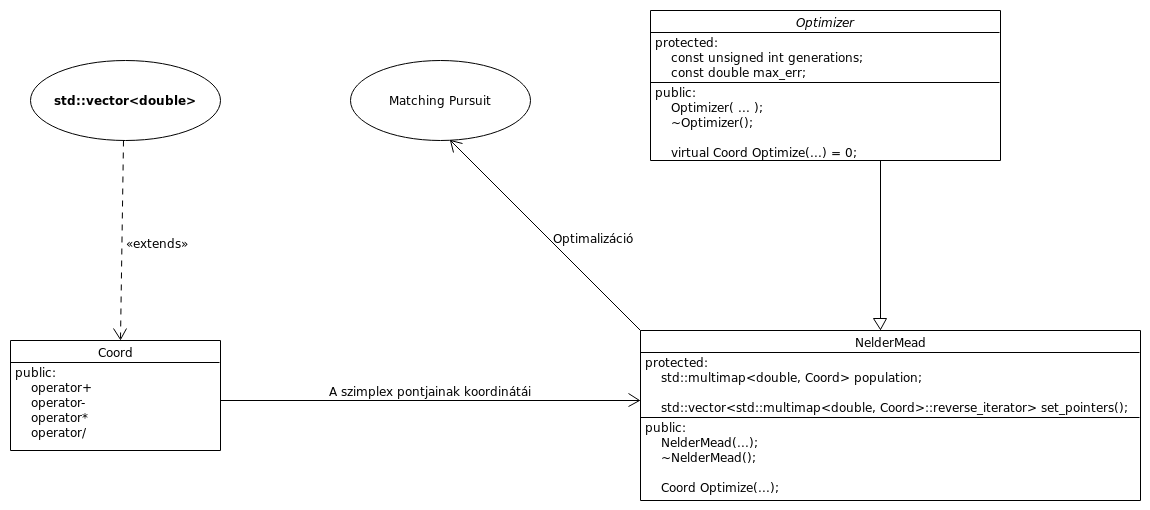
\includegraphics[scale=0.25]{./figures/NelderMead.png}
		\caption{A NelderMead modul UML diagrammja}
	\end{center}	
\end{figure}

\end{frame}

\begin{frame}{A felhasználói felület}
\linespread{0.8}
\small
\vspace{-2mm}
\begin{block}{Alkalmazott technikák}
	\begin{itemize}
		\item Feladatspecifikus nyelvválasztás. Felhasznált programnyelvek: php, javascript, bash.
		\item Külső technológiák integrálása: GoogleCharts, jQuerry.
	\end{itemize}
	\end{block}		
	
\begin{block}{Kényelem orientált felépítés}
	\begin{itemize}
		\item Átlátható horizontális menüsor.
		\item Ismertető felület.
		\item Esztétikus megjelenés. Tervező grafikus által szerkesztett külalak. 
	\end{itemize}
\end{block}		

\end{frame}

\begin{frame}{A felhasználói felület}
\linespread{0.8}
\small
\vspace{-2mm}

\begin{figure}[H]
\begin{center}
   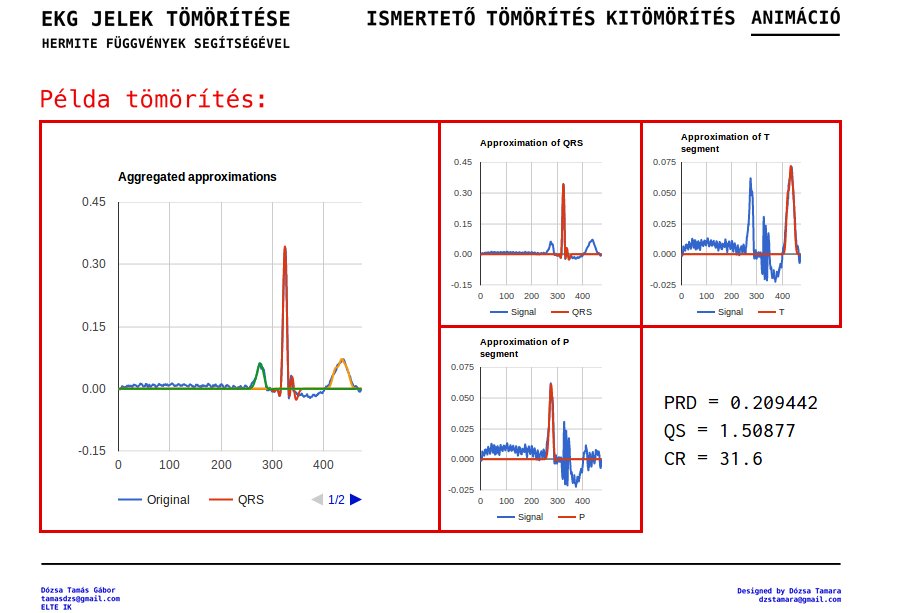
\includegraphics[scale=0.25]{./figures/animpage.png}
   \caption{Az animation.php}
\end{center}
\end{figure}

\end{frame}


\begin{frame}{A fejlesztés jellemzése}
\linespread{0.8}
\small
\vspace{-2mm}
\begin{block}{A rendszer felépítése}
	\begin{itemize}
		\item Könnyű telepítés, fordítás.
		\item Logikus könyvtár felépítés. 
		\item Kód, modul tesztek, webes tartalom elszeparálása.
		\item Verziókezelő rendszer (git) alkalmazása.
	\end{itemize}
	\end{block}		
	
\begin{block}{A kód jellemzése}
	\begin{itemize}
		\item Azonos kódolási stílus használata. 
		\item Konstans értékek használata. "Varázsszámok" szűrése.
		\item Beszédes azonosítók használata. (pl. t\_inActionSig\_ofs).
	\end{itemize}
	\end{block}
\end{frame}

\section{Tesztek, eredmények}
\label{tab:results}

\begin{frame}{A programcsomag tesztelése}
\linespread{0.8}
\small
\vspace{-2mm}
\begin{block}{Modul tesztek}
	\begin{itemize}
		\item Minden modulhoz külön modulteszt.
		\item Eredmények, modulteszt kódja: ./src/mt/[modul neve]
	\end{itemize}
	\end{block}		
\end{frame}

\begin{frame}{Tesztelés}
\only<1>{
\begin{block}{Értékelés}
	\begin{itemize}
		\item Percentage root mean square difference (PRD):
			\begin{equation*}
					\PRD=\frac{\left\|S_{n}^{a,\lambda}f-f\right\|_2}{\left\|f-\conj{f}\right\|_2}\times 100\,.  		
			\end{equation*}		
		\item Compression ration (CR):
			\begin{equation*}
				\CR=\frac{\text{eredeti EKG mérete}}{\text{tömörített EKG mérete}}\times 100\,.
			\end{equation*}		
		\item Quality score (QS):
			\begin{equation*}
				\QS=\frac{CR}{PRD}\,.
			\end{equation*}		
	\end{itemize}
\end{block}
}
\only<2>{
	\begin{block}{Technikai adatok}
		\begin{itemize}
			\item PhysioNet EKG adatbázisból $6$ egyenként fél órás rekordon.
			\item $12830$ szívütés, rekordonként 1400-1600 másodperces futásidő.
		\end{itemize}
	\end{block}
\begin{table}[H]
\scriptsize
\centering
	\scalebox{0.7}{
\begin{tabular}{|c||cccc|cccc|cccc|}
\multicolumn{1}{c}{} & \multicolumn{4}{c}{\textbf{Hiba (PRD \%)}} & \multicolumn{4}{c}{\textbf{A t\"om\"or\'\i t\'es ar\'anya (CR $1:X$)}} & \multicolumn{4}{c}{\textbf{Quality Score ($\CR:\PRD$)}}\bigstrut\\\hline
\textbf{Rec.} & \textbf{Eredeti} & \textbf{NM} & \textbf{PSO} & \textbf{JPEG2} & \textbf{Eredeti} & \textbf{NM} & \textbf{PSO} & \textbf{JPEG2} & \textbf{Eredeti} & \textbf{NM} & \textbf{PSO} & \textbf{JPEG2} \bigstrut[t]\\
101 & 11.20 & 11.10 & 11.13 &11.07& 29.71 & 27.22 & 27.22 & 18.94 &\textbf{2.65}&2.45&2.47& 1.71\\
117 & 13.20 & 11.81 & 17.66 &11.66& 36.07 & 33.06 & 33.06 & 23.66 &2.73&\textbf{2.79}&1.87& 2.02\\
118 & 19.83 & 17.79 & 16.65 &17.72& 24.34 & 22.30 & 22.30 & 32.91 &1.22&1.25&1.33& \textbf{1.85}\\
\textcolor{red}{119} & \textcolor{red}{14.27} & \textcolor{red}{8.76} & \textcolor{red}{10.20}  &\textcolor{red}{8.80} & 27.89 & 25.55 & 25.55 & 23.85 &1.95&\textbf{2.91}&2.51& 2.71\\
201 & 13.51 & 12.17 & 12.17 &12.14& 28.21 & 25.35 & 25.35 & 13.15 &\textbf{2.08}&\textbf{2.08}&\textbf{2.08}& 1.08\\
213 & 19.92 & 18.28 & 17.60 &18.29& 17.08 & 15.64 & 15.64 & 35.23 &0.85&0.85&0.88& \textbf{1.92}\\
%214 & 7.61 & 7.90 & 11.40   &7.91 & 24.53 & 22.04 & 22.47 & 19.32 &&&&\\
\hline
\textbf{\'Atlag} & 14.22 & 12.55 & 13.83 &12.51& 26.83 & 24.45 & 24.51 & 23.86 &1.91&\textbf{2.06}&1.85& 1.88\\\hline
\end{tabular}
}
\caption{A tömörítés \"osszehasonl\'\i t\'asa k\"ul\"onb\"oz\H o m\'odszerek eset\'en.}
\label{tab:results}
\end{table}
}
\only<3>{
\begin{figure}[htb!]
  \centering
\subfigure[Eredeti módszer.]{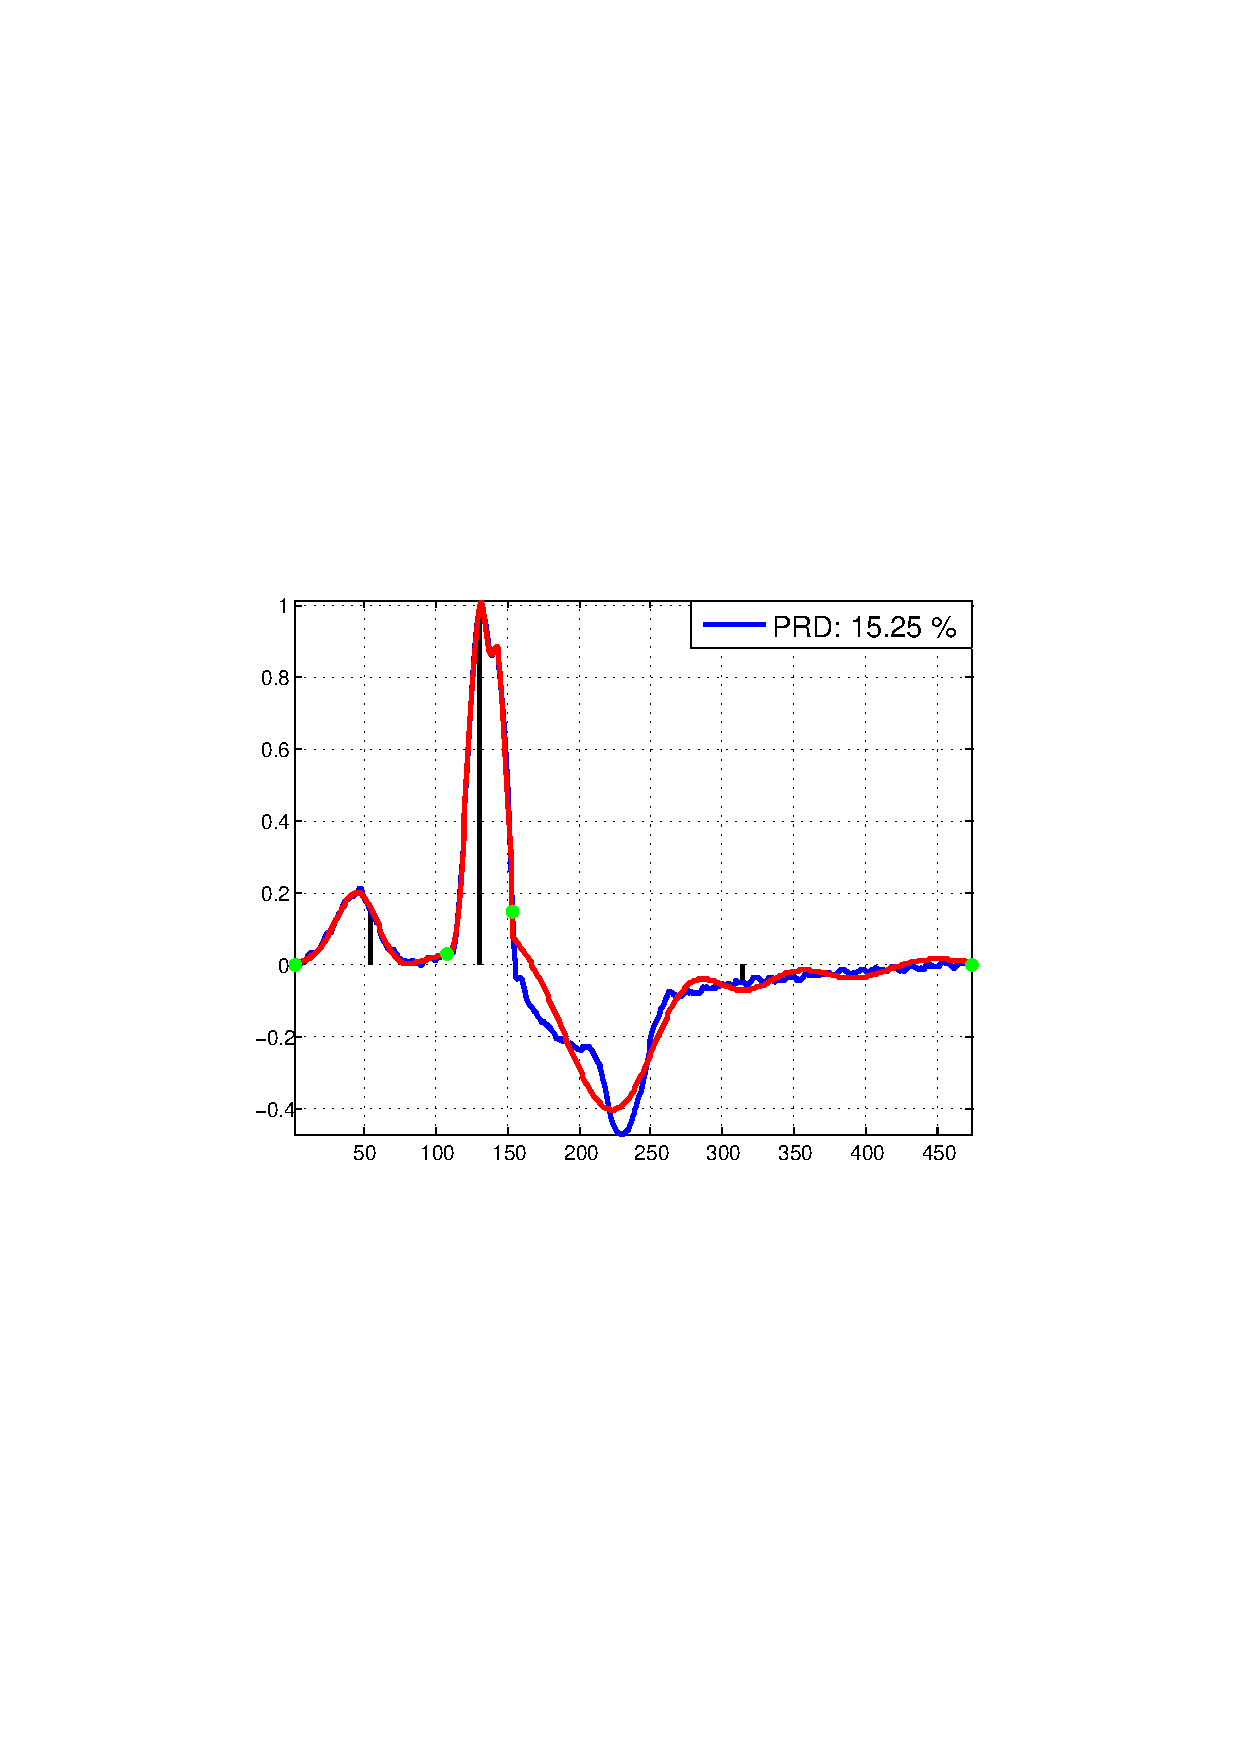
\includegraphics[scale=0.4,trim=120 280 100 280,clip]{./figures/eredeti_abra1.pdf}}\hspace{1mm}
\subfigure[Saját módszer.]{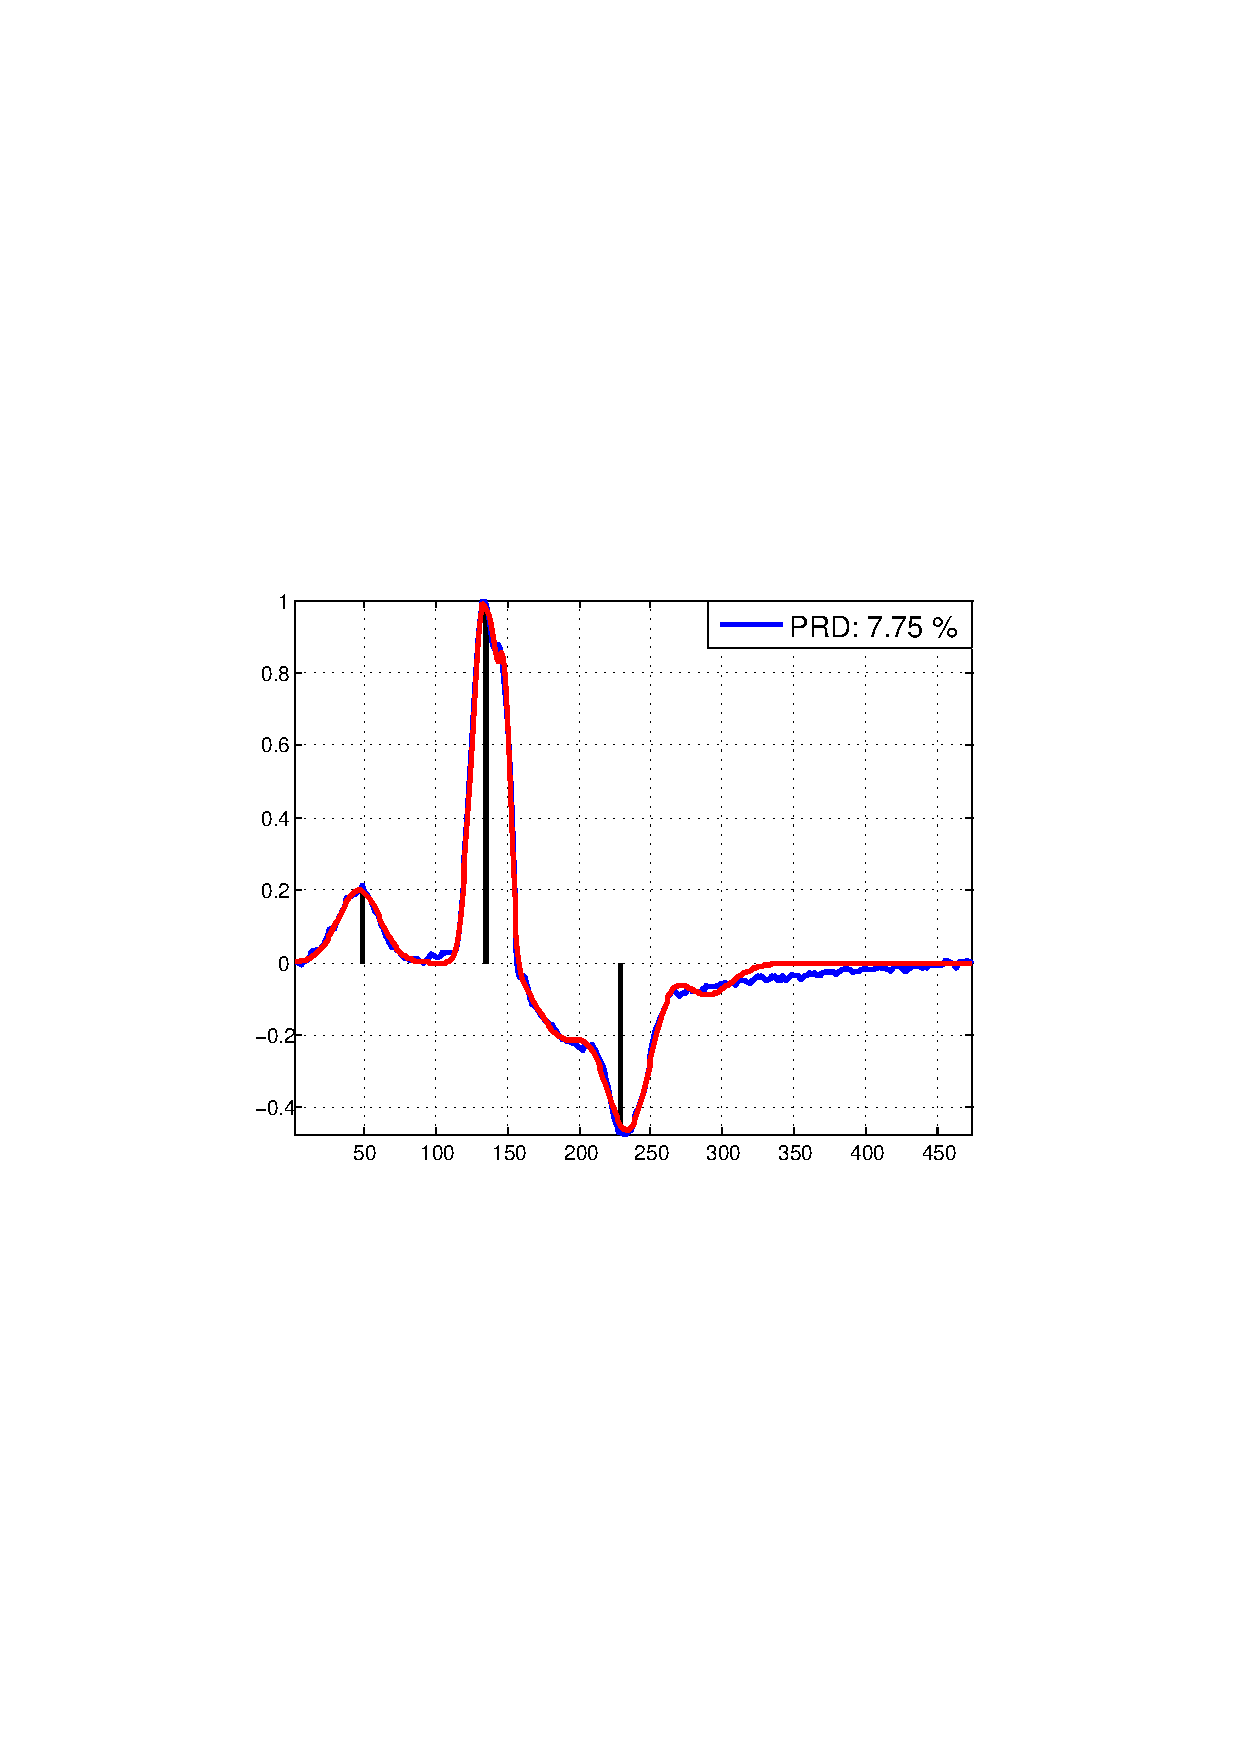
\includegraphics[scale=0.4,trim=120 280 100 280,clip]{./figures/sajat_abra1.pdf}}
\caption{Asszimetrikus EKG jel közelítése (119-es rekord).}
\end{figure}
}
\end{frame}

\begin{frame}{Más algoritmusokkal való összehasonlítás}
	\begin{figure}
	\subfigure[180 szomszédos szívütés.]{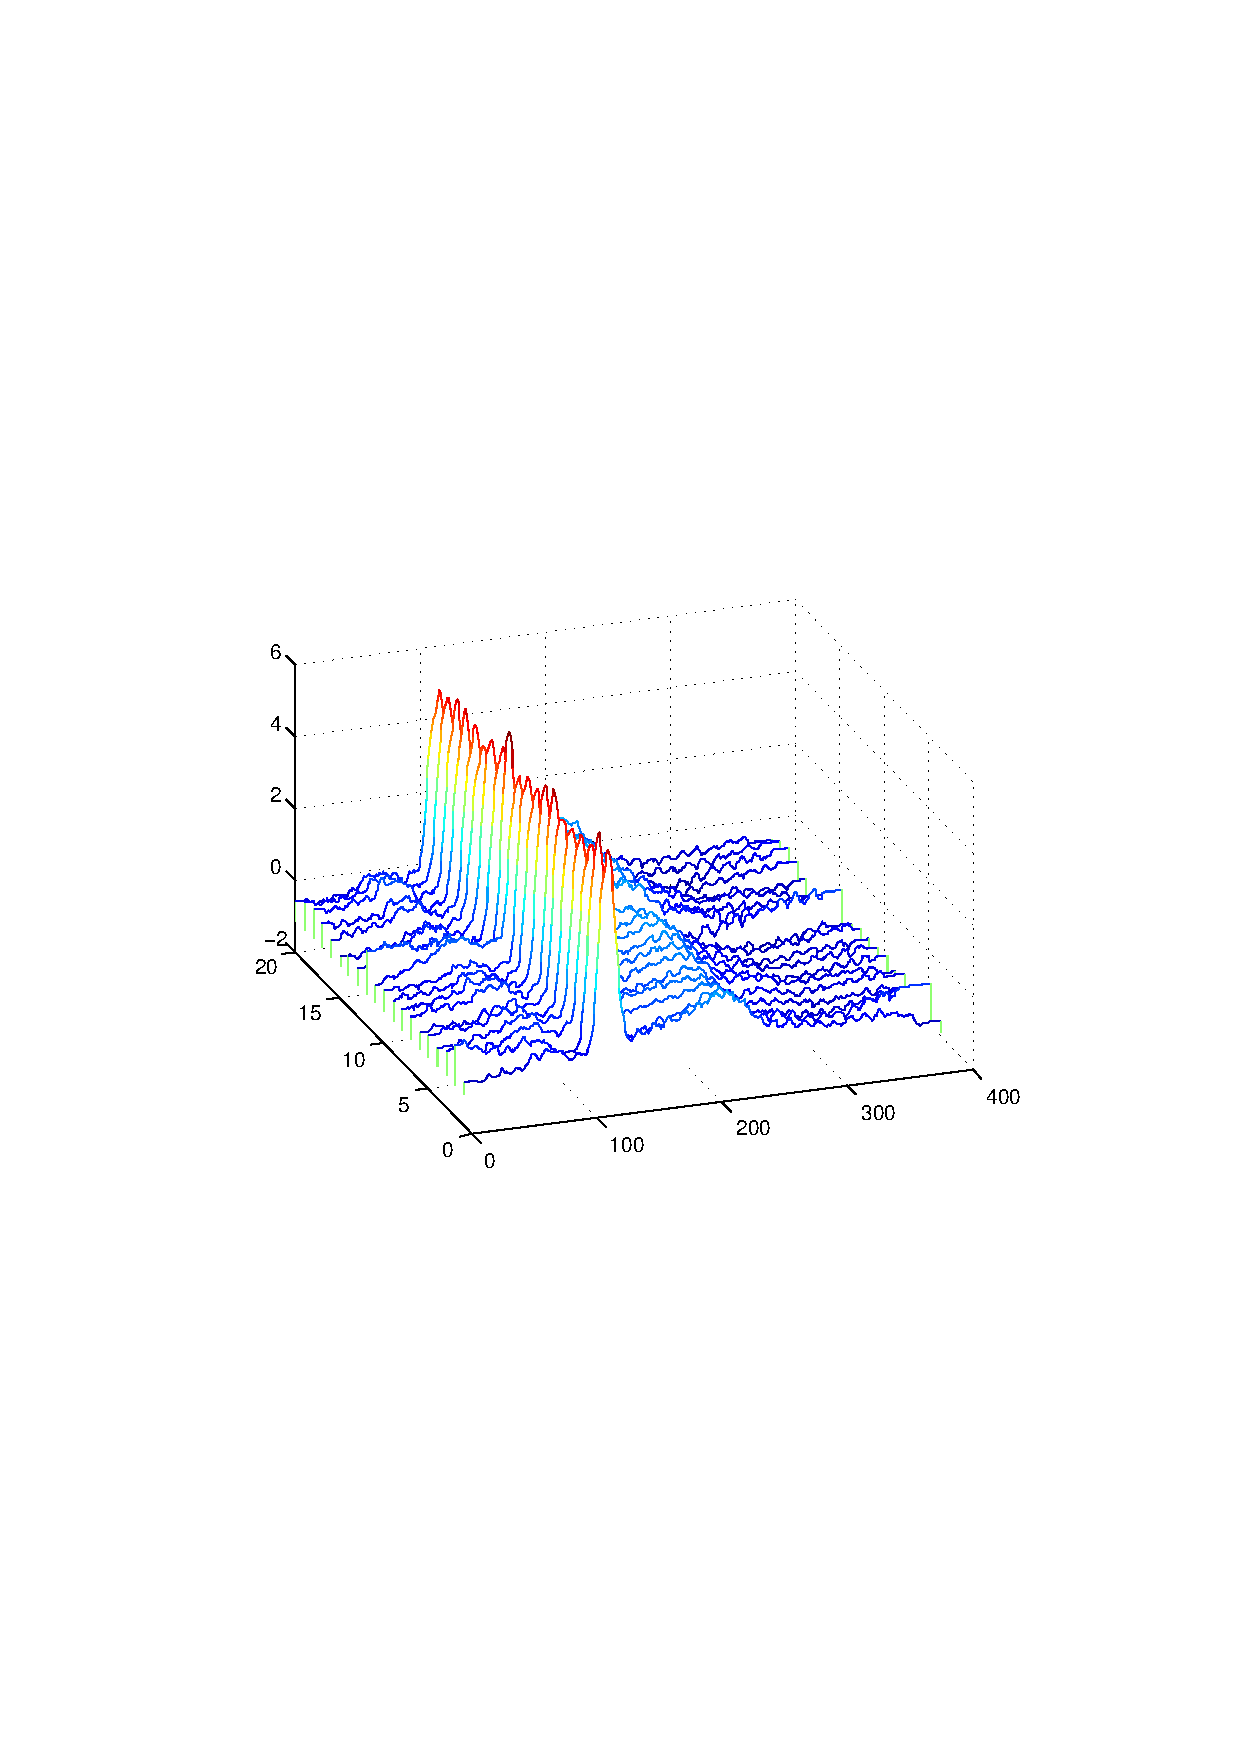
\includegraphics[scale=0.38,trim=100 280 100 280,clip]{./figures/waterfall_ECG.pdf}}
	\subfigure[Szívütések 2D képe.]{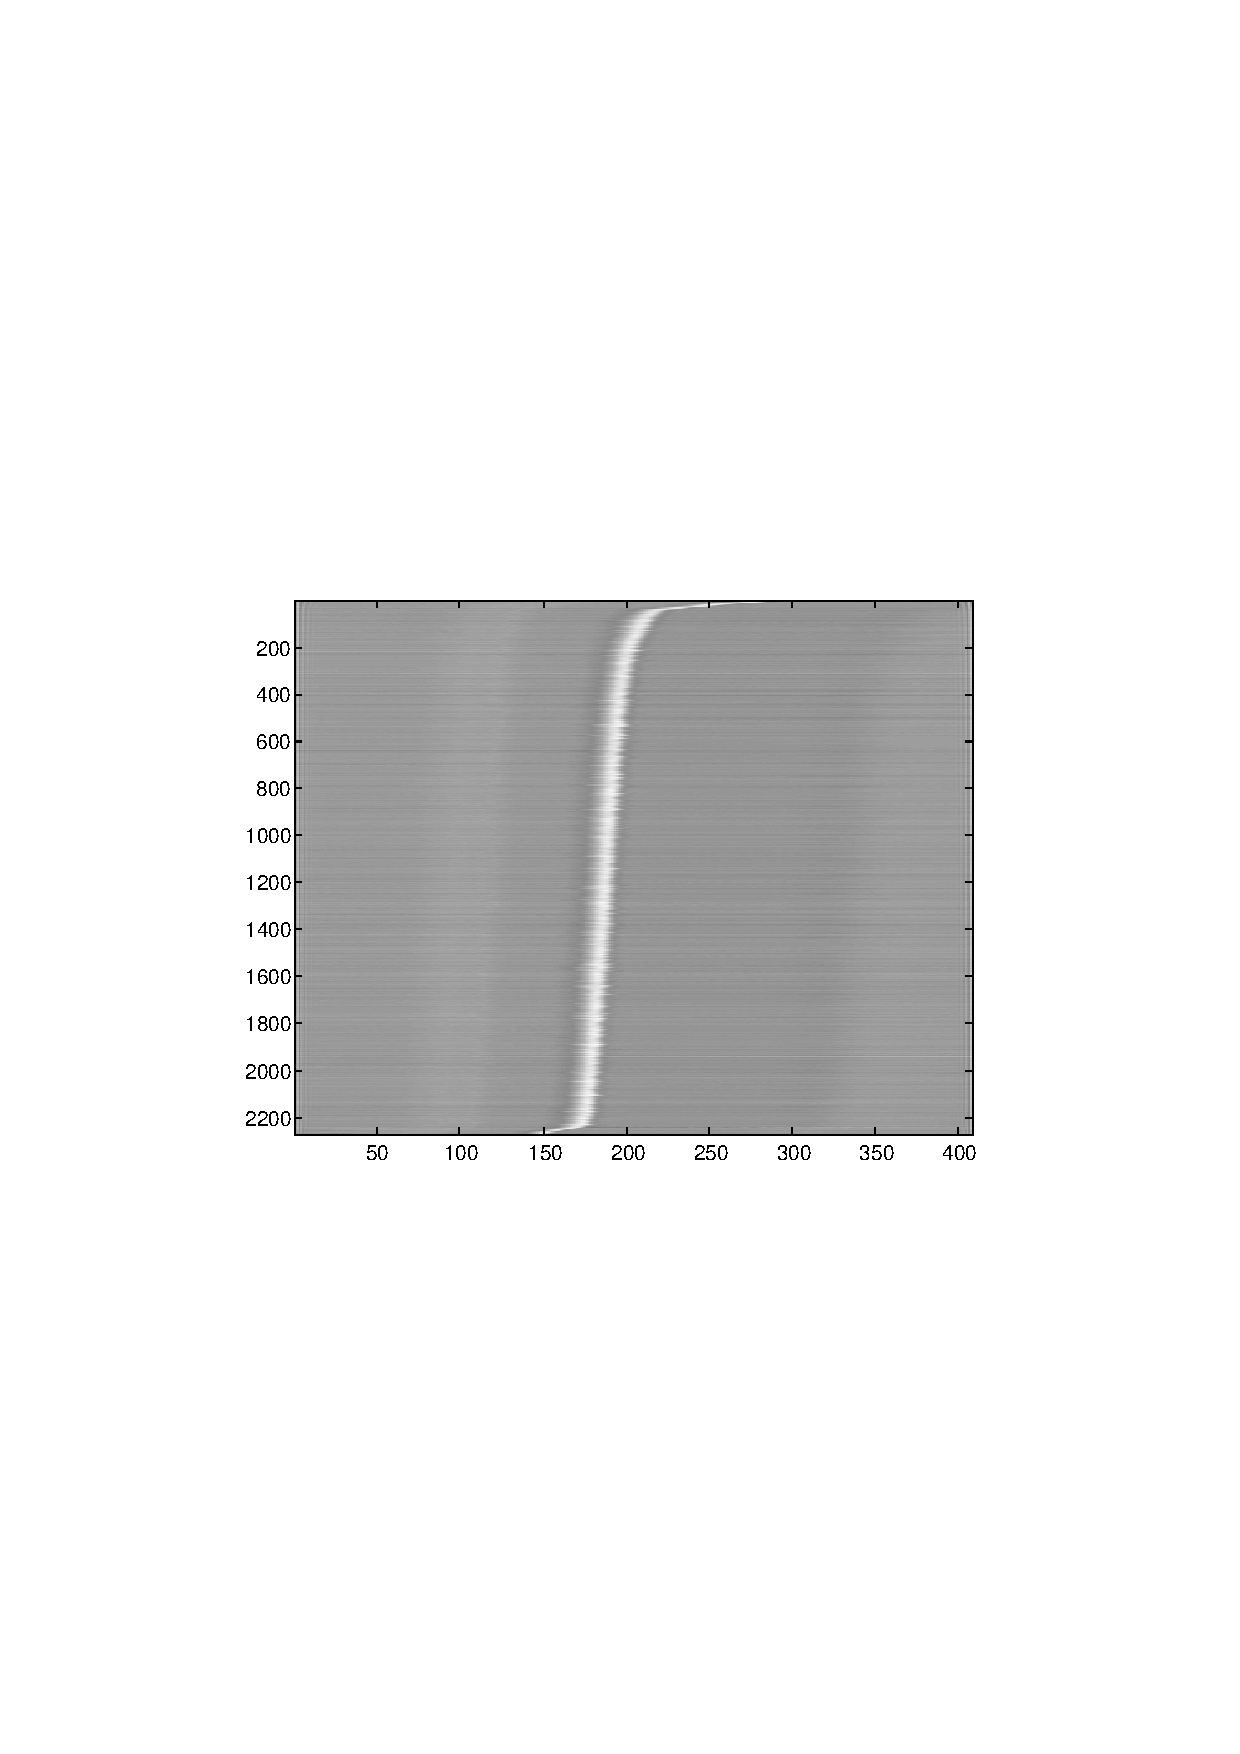
\includegraphics[scale=0.38,trim=100 280 100 280,clip]{./figures/ecg2d.pdf}}
	\caption{EKG jelek feldolgozása képtömörítő algoritmusok segítségével.}
\end{figure}
\end{frame}

\begin{frame}{Összefoglalás}
\linespread{0.8}
\small
\vspace{-2mm}
\begin{block}{Eredmények}
	\begin{itemize}
		\item Új ONR szerkesztése transzlációval és dilatációval.
		\item Optimum létezésének belátása.
		\item Alkalmazás EKG jelek tömörítésére, szegmentálására.
		\item Tesztelés valós adatsorozatokon.
		\item Hatékony implementáció elkészítése, webes felhasználói felülettel.
		\item Összehasonlítás más módszerekkel: fix Hermite, JPEG2000.
		\item Módszer publikálása nemzetközi folyóiratban \cite{sajat}.
	\end{itemize}
	\end{block}				
	\begin{block}{Konklúzó}
	\begin{itemize}
		\item A módszer hatékonyan alkalmazható EKG jelek tömörítésére.
		\item Pontosabb közelítés érhető el asszimetrikus jelek esetén.
		\item Közel valósidejű feldolgozás lehetséges.	
	\end{itemize}
	\end{block}	
\end{frame}

\begin{frame}{Irodalomjegyzék}
\begin{thebibliography}{9}
\linespread{1.0}

\bibitem{Szoke} B.~Szokefalvi-Nagy, \lq\lq Valós függvények és függvénysorok,\rq\rq~in~\emph{Polygon Könyvtár}, Szeged, HU, 2002.

\bibitem{Szego} G.~Szeg\H{o}, \lq\lq Orthogonal polynomials,\rq\rq~\emph{AMS Colloquium Publications}, New York, USA, 3rd edition, 1967.

\bibitem{Gautschi} W.~Gautschi, \lq\lq Orthogonal Polynomials, Computation and Approximation,\rq\rq~in~\emph{Numerical Mathematics and Scientific Computation}, Oxford University Press, Oxford,
UK, 2004.

\bibitem{Mallat} S.~G.~Mallat, Z.~Zhang, \lq\lq Matching pursuit in time-frequency dictionary,\rq\rq~in~\emph{IEEE Transactions on Signal Processing}, vol. 41, no. 12, pp. 3397–3415, 1993.

\bibitem{sajat} 
T. Dozsa, P. Kovacs,
„ECG Signal Compression Using Adaptive Hermite Functions,”
\textit{ Advances in Intelligent Systems and Computing},
AISC, volume 399

%\bibitem{PhysioNet} A.~L.~Goldberger, L.~A.~N.~Amaral, L.~Glass, J.~M.~Hausdorff, P.~Ch.~Ivanov,
%R.~G.~Mark, J.~E.~Mietus, G.~B.~Moody, C.~K.~Peng, and H.~E.~Stanley, \lq\lq PhysioBank,
%PhysioToolkit, and PhysioNet: Components of a new research resource
%for complex physiologic signals,\rq\rq~in~\emph{Circulation}, vol. 101, no. 23, pp. 215–220, 2000.

\end{thebibliography}
\end{frame}

\begin{frame}{}
\end{frame}


\begin{frame}{Kitekintés}
\begin{figure}[htb!]
  \centering
\subfigure[Rossz eset.]{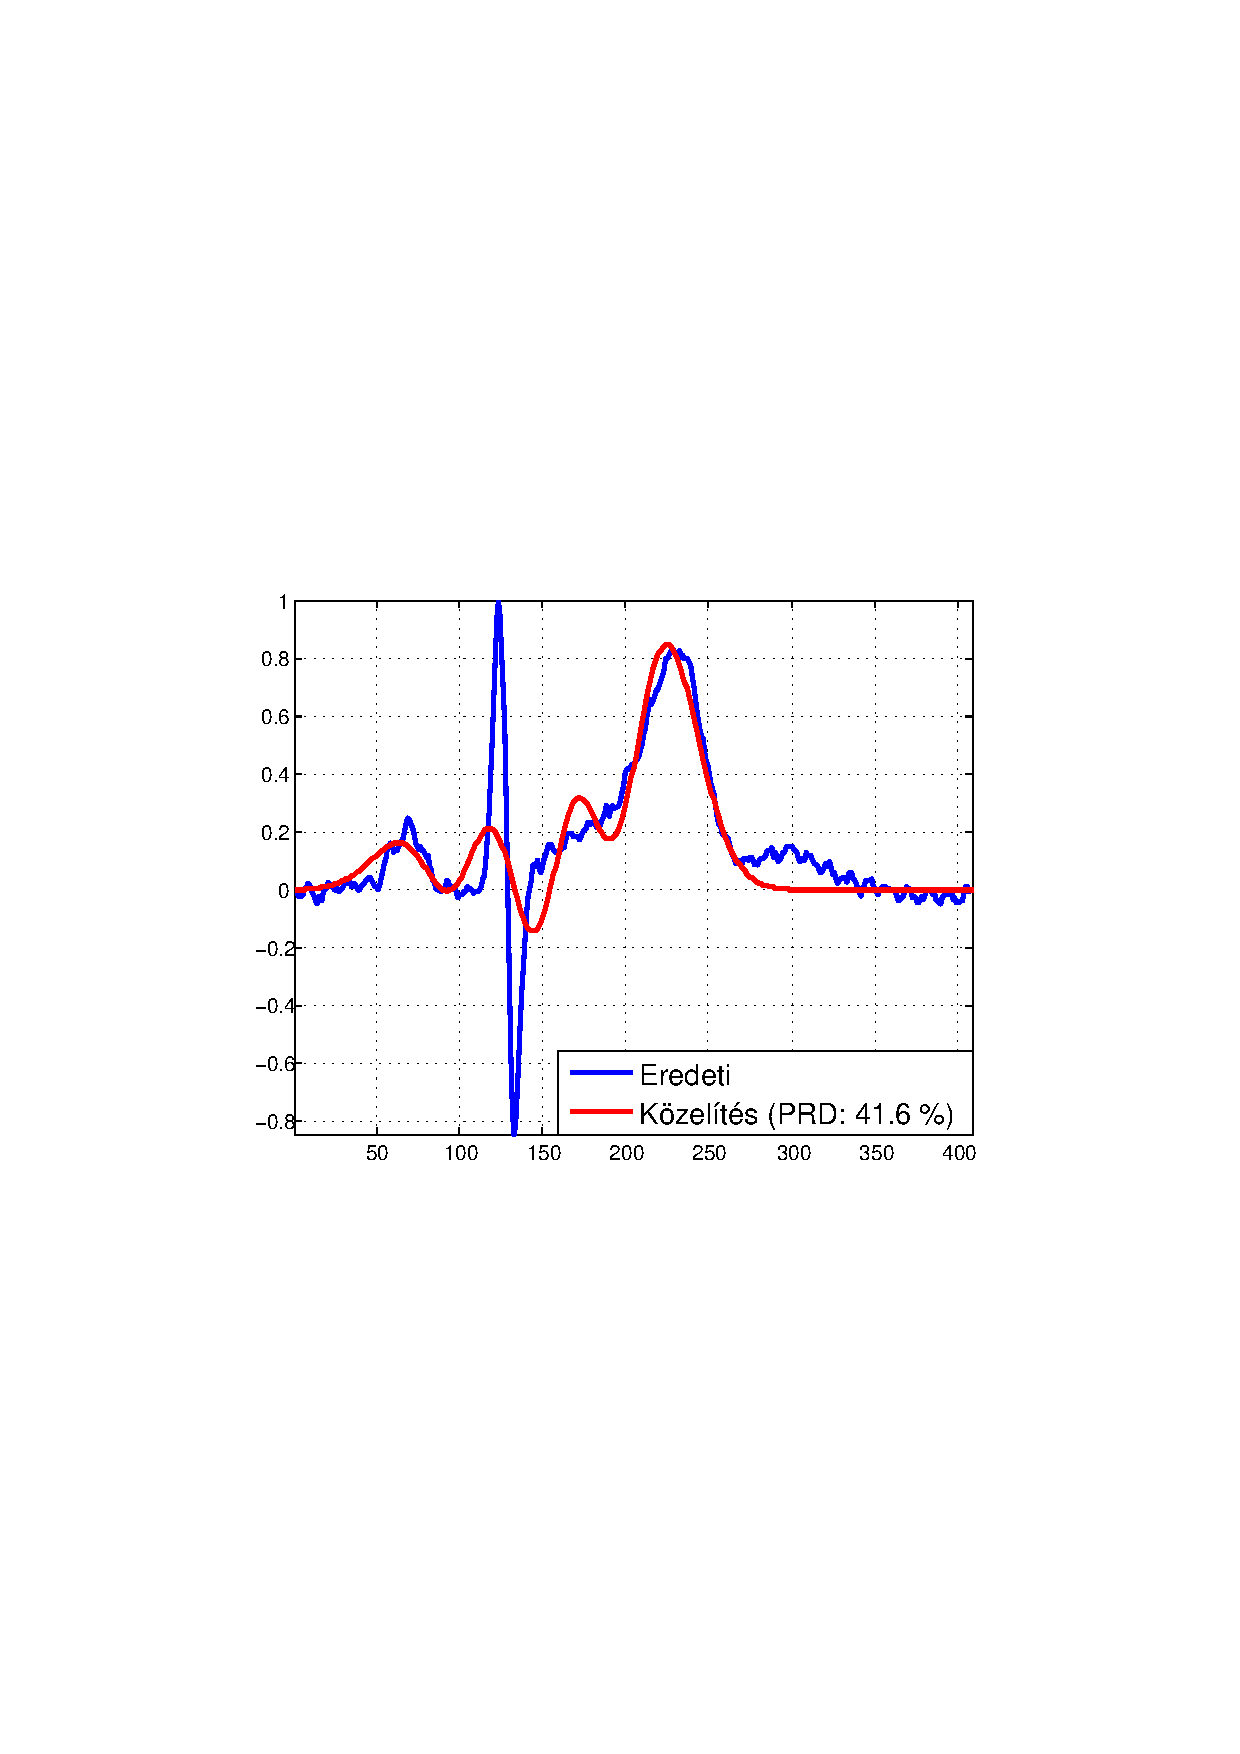
\includegraphics[scale=0.38,trim=100 280 100 280,clip]{./figures/abra762_bad.pdf}}
\subfigure[Jó eset.]{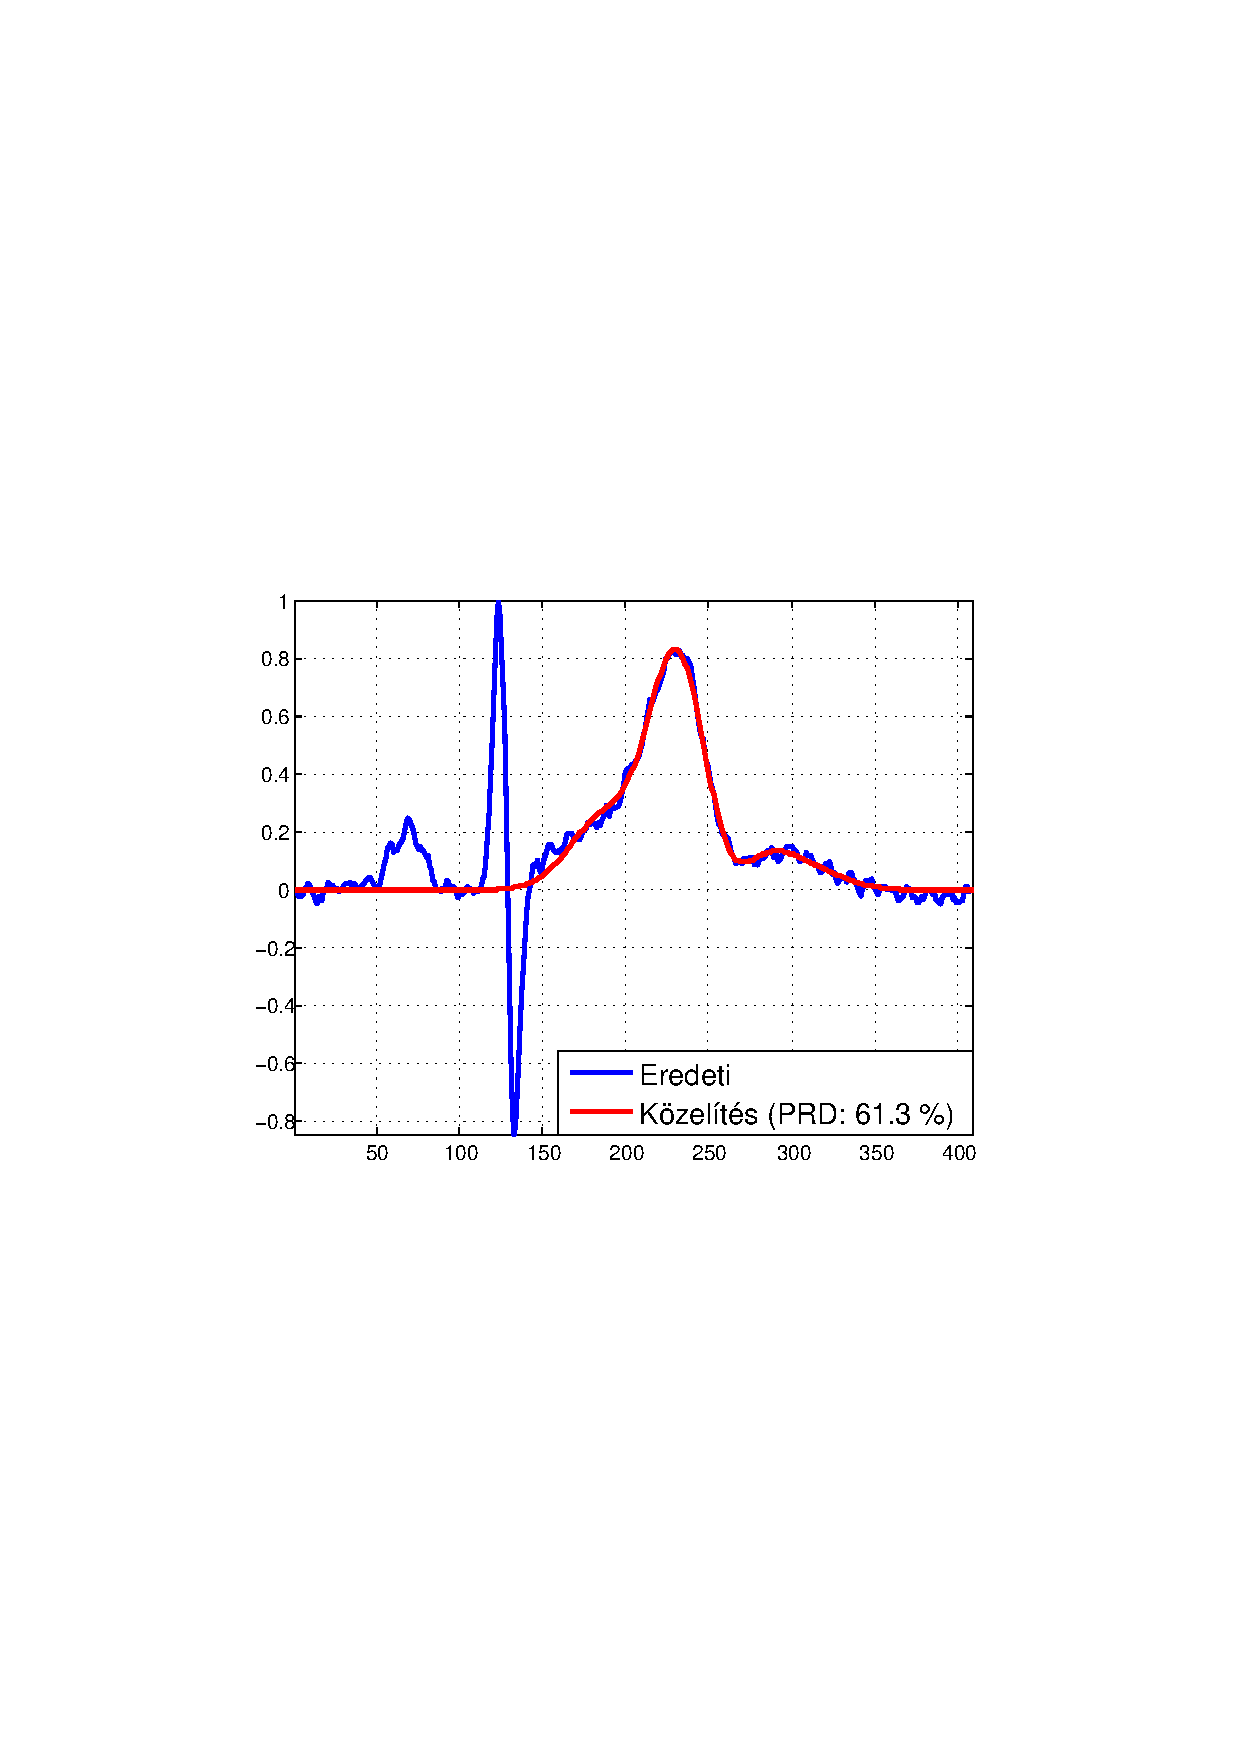
\includegraphics[scale=0.38,trim=100 280 100 280,clip]{./figures/abra762_good.pdf}}
\caption{A mohó stratégia hátránya.}
\end{figure}
\end{frame}

\begin{frame}{Nelder--Mead szimplex módszer}
\only<1>{
	\begin{block}{Cél}
		A $D^2_n(a,\lambda)$ hibafüggvény minimumhelyének meghatározása.
				%\begin{equation*}
					%D^2_n(a,\lambda):=\|f\|^2-\sum_{k=0}^n|\langle f,\Phi_k^{a,\lambda}\rangle|^2\,.
				%\end{equation*}
	\end{block}
	\begin{block}{Algoritmus}
		\begin{itemize}
			\item Kizárólag az $ f(x_3)\le f(x_2)\le f(x_1)$ értékekre támaszkodik.
			\item Keressük az $x'=x_1+\alpha (x-x_1)\ \ (\alpha\in\Bbb R)$ pontot, melyre
			\begin{equation*}
				f(x')\le f(x_2)\le f(x_1)\,,
			\end{equation*}
			ahol $x=(x_2+x_3)/2$ a két kisebb érték között húzott szakasz felezőpontja.
		\end{itemize}
	\end{block}
	}
\only<2>{
\small
\linespread{0.8}
		\begin{block}{Geometriai transzformációk}
		\begin{itemize}
			\item $\alpha=2$ esetén pont egy $x$-re vonatkozó középpontos tükrözés ($T_1$).
			\item $\alpha>2$ esetén a tükrözés és nyújtás $(T_2)$.
			\item $1<\alpha<2$ esetén tükrözés és zsugorítás $(T_3)$.
			\item $-1<\alpha<0$ esetén egyszerű zsugorítás ($T_4$). 
		\end{itemize}
	\end{block}
\vspace{-3mm}
\begin{figure}[htb!]
  \centering
\subfigure[T\"ukr\"oz\'es\ $(T_1: \alpha=2).$]{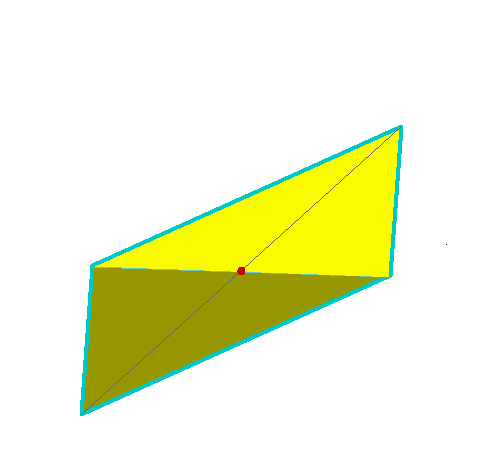
\includegraphics[scale=0.22,trim=10 0 10 53,clip]{./figures/NMT1.PNG}} \hspace{10mm}
\subfigure[T-Ny\'ujt\'as\ $(T_2: \alpha=2.5).$]{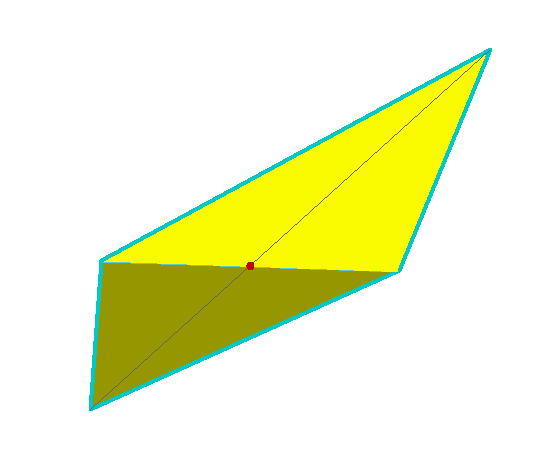
\includegraphics[scale=0.22,trim=10 0 10 53,clip]{./figures/NMT2.PNG}}
\end{figure}
}
\only<3>{
\small
\linespread{0.8}
\begin{figure}[htb!]
\subfigure[T-\"Osszeh\'uz\'as\  $(T_3:  \alpha=1.5).$]{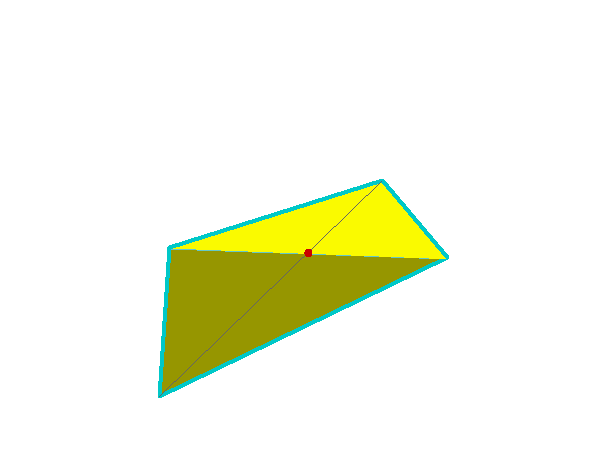
\includegraphics[scale=0.22,trim=10 0 10 53,clip]{./figures/NMT3.PNG}} 
\subfigure[Összeh\'uz\'as\ $(T_4: -1<\alpha<0).$]{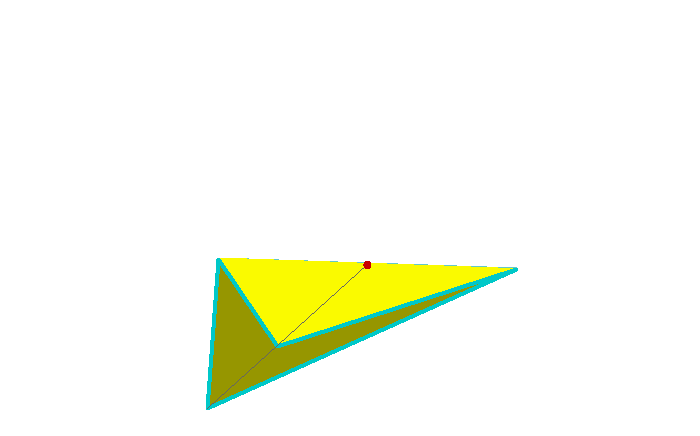
\includegraphics[scale=0.22,trim=10 0 10 185,clip]{./figures/NMT4.PNG}}
\subfigure[Kicsiny\'\i t\'es  $x_3$-b\'ol $(T_5).$]{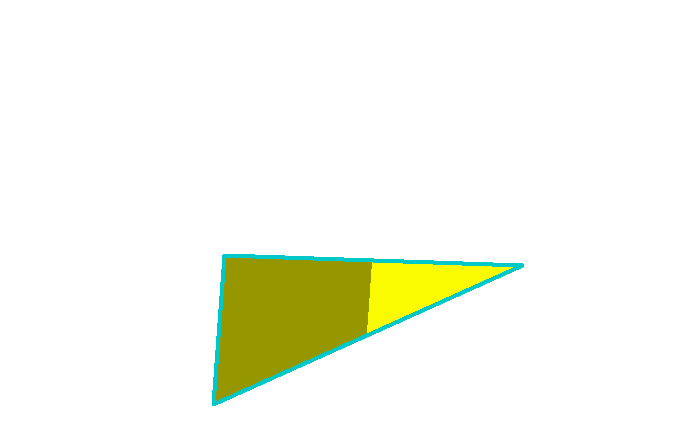
\includegraphics[scale=0.22,trim=10 0 10 185,clip]{./figures/NMT5.PNG}}
\end{figure}
}
\end{frame}

\begin{frame}{Diagnosztikai torzulás jellemzése}
\only<1>{
\linespread{1.0}
	\begin{block}{Alternatívák}
	\begin{itemize}
		\item WDD (2000): orvosdiagnosztikában használt jellemzők közvetlen átvétele \footnotemark[1].
			\begin{itemize}
				\item Hátrány: a felhasznált feature-k detektálása nagyon nehéz. 
			\end{itemize}
		\item WWPRD (2006): wavelet együtthatók súlyozott PRD-je \footnotemark[2].
   		\begin{itemize}
				\item Előny: könnyen implementálható, csak QRS detektálás szükséges.
			\end{itemize}
	\end{itemize}
	\end{block}
\footnotetext[1]{Y. Zigel, A. Cohen, and A. Katz, \textit{The Weighted Diagnostic Distortion (WDD) Measure
for ECG Signal Compression}, IEEE Trans. on Biomed. Eng., vol. 47, no. 11, pp. 1422--1430, 2000. \vspace{3mm}}
	
\footnotetext[2]{A. S. Al-Fahoum, \textit{Quality Assessment of ECG Compression Techniques Using a Wavelet-Based Diagnostic Measure}, IEEE Trans. on Inf. Tech. in Biomed., vol. 10, no. 1, pp. 182--191, 2006. \vspace{3mm}}	
}

\only<2>{
%	\begin{block}{Diagnostic Features (WDD)}
%		$RR_{int}, QRS_{dur}, QT_{int}, QTp_{int}, P_{dur}, PR_{int}, QRS_{peaks}, QRS_{sign}, \Delta_{wave?},$
%		$T_{shape}, P_{shape}, ST_{shape}, QRS^+_{amp}, QRS^-_{amp}, P_{amp}, T_{amp}, ST_{elevation}, ST_{slope}$
%	\end{block}	
	\begin{figure}
		\begin{center}
			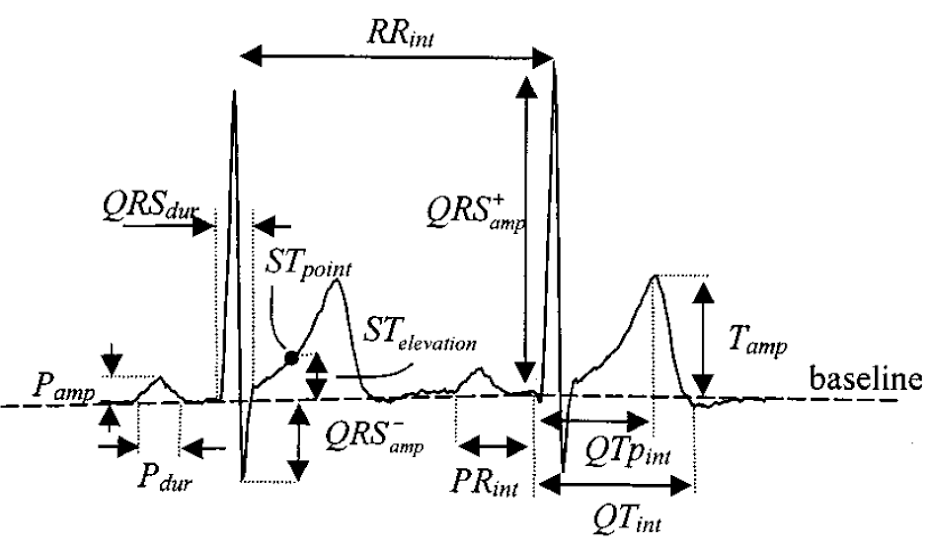
\includegraphics[scale=0.27]{./figures/ECGfeatures.png}
		\end{center}
		\caption{Egy szívütés diagnosztikai jellemzői (WDD).}
	\end{figure}	
}
\only<3>{
\begin{table}[t!]
\centering
\scriptsize
\begin{center}
	\begin{tabular}{|c|c|c|c|c|c|} \hline
		\multirow{2}{*}{\textbf{Mérték}} & \multicolumn{5}{|c|}{\textbf{Minősítés}} \\ \cline{2-6}
		\textbf{} & \textbf{Tökéletes} & \textbf{Nagyon jó}  & \textbf{Jó} & \textbf{Nem Rossz} & \textbf{Rossz} \\ \hline
		\textbf{PRD} & 0-4.33 & 4.33-7.8 & 7.8-11.59 & 11.59-22.5 & $22.5<$ \\ \hline
		\textbf{$\text{WWPRD}_h$} & 0-7.4 & 7.4-15.45 & 15.45-25.18 & 25.18-37.4 & $37.4<$\\ \hline
	\end{tabular}
\end{center}
\label{tab:quality_pred}
\caption{Tömörítés diagnosztikai minősége PRD és $\text{WWPRD}_h$ alapján.}
\end{table}
}
\end{frame}
\end{document}



